\chapter{INTRODUCTION ABOUT MPIC SYSTEM}

\renewcommand{\headrulewidth}{0.5pt}
\renewcommand{\footrulewidth}{0.5pt}
\thispagestyle{plain}
\pagestyle{fancy}
\fancyhf{}
\fancyhead[L]{\textbf{CHAPTER 4}}
\fancyhead[R]{\textbf{Graduate Report}}
\raggedright
\fancyfoot[L]{From: Nguyen Van Anh Tuan}
\fancyfoot[R]{Page \thepage}

\justifying

\section{Simulation Interface Concept}
    \subsection{What is an interface module?}
        It is the module that allow the software to control and to monitor the cockpit hardware.
    \subsection{MPIC Interface System Overview Software Module}
        \begin{figure}[H]
            \centering
            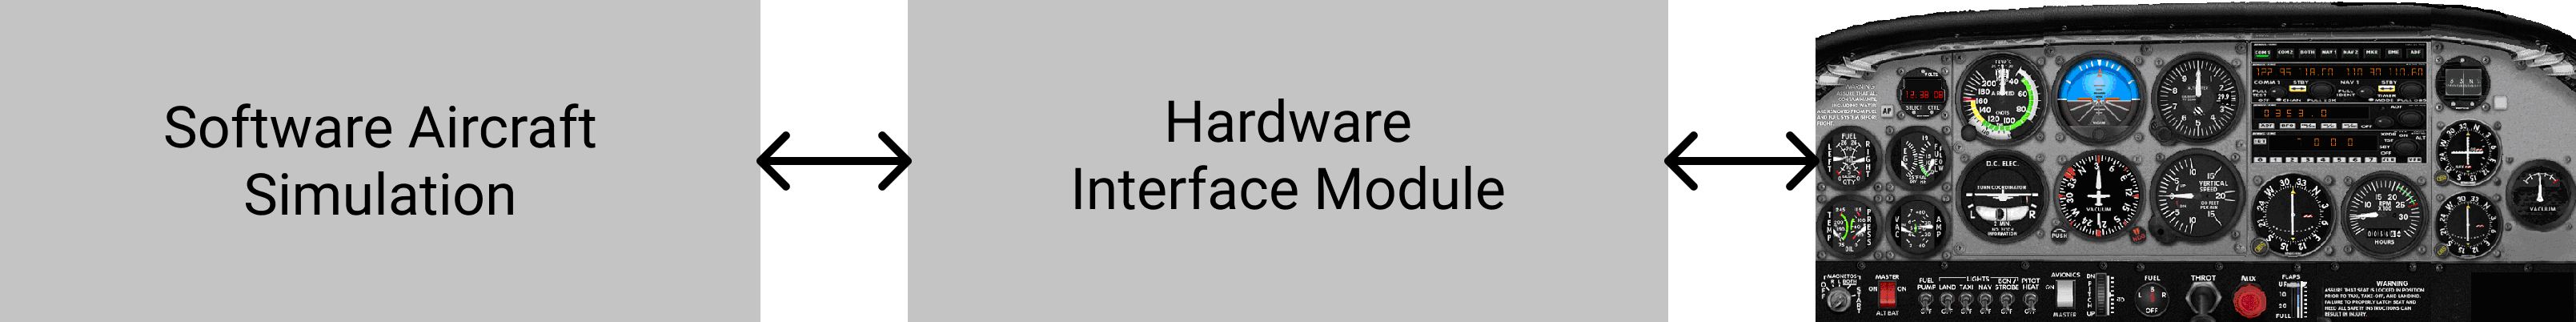
\includegraphics[width=0.6\linewidth]{img/MPIC.png}
            \caption{MPIC Interface System Overview Software Module}
        \end{figure}
        \begin{figure}[H]
            \centering
            \includegraphics[width=0.6\linewidth]{img/simulator-support-system.png}
            \caption{Simulator Support Systems}
        \end{figure}

\section{Interface System Architecture}
    \subsection{Architecture Overview}
        To meet the A661 standard used by CAE, we must seperate the User Application (UA) from the Cockpit Display System (CDS). 
        In other words, the appearance and contents of an object (Widget) on the display must be segregated from its functional 
        behavior as this is managed by the UA. As a result, the system structure can be divided into two main modules, as shown 
        in below figure, specifically the PC where the simulator sends all the data to be processed by the UA, and the CAE-MPIC 
        where the graphics rendering is performed. \\ 
        \vspace{3mm}
        To make things simple we choose to categorize the architecture into four modules:
        \begin{itemize}
            \item The UA
            \item The CDS 
            \item The Window Manager UA
            \item The communication protocol ARINC 661/DUP
        \end{itemize}
        \begin{figure}[H]
            \centering
            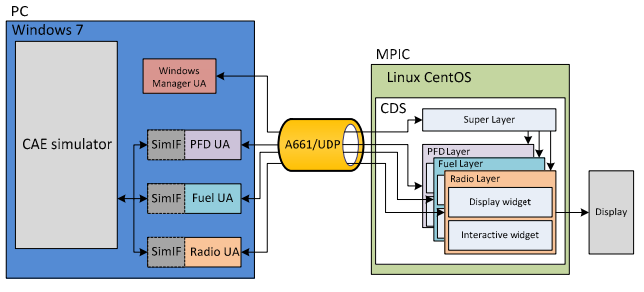
\includegraphics[width=0.6\linewidth]{img/UA.PNG}
            \caption{System Architecture}
        \end{figure}
    \subsection{What Is ARINC 661?}
        ARINC 661 is a standard which aims to normalize the definition of a \textbf{C}ockpit \textbf{D}isplay \textbf{S}ystem (CDS), 
        and the communication between the CDS and User Applications (UA) which manage aircraft avionics functions. The GUI definition 
        is completely defined in binary \textbf{D}efinition \textbf{F}iles (DF).\\
        \vspace{3mm}
        The CDS software is constituted of a kernel which is able to create the GUI hierarchy specified in the DF during initialization, 
        thus not needing to be recompiled if the GUI definition changes. \\
        \vspace{3mm}
        The standard normalizes: 
        \begin{itemize}
            \item the GUI definition of the CDS interface, in a binary file called DF (Definition File) defining the structure of the 
            graphical interface tree. The GUI tree is instantiated at initialization time (called the Definition Phase in the standard) 
            in the CDS, using the definition contained in the DF;
            \item the communication at runtime between the User Applications (UA) and the CDS. This communication protocol is typically 
            used for UAs to send widgets modifications to the CDS, and return user events (such as buttons selection) from CDS to UA.
        \end{itemize}
        In order to be compliant with the standard, a CDS must have a kernel that can create the widgets tree during CDS initialization, 
        using the Definition File, and communicate with UA in both ways using the runtime protocol. \\ 
        \vspace{3mm}
        ARINC 661 does not imply the use of a particular Data bus structure to perform the low-level communication between CDS and UA. 
        For example, an ARINC 429 or Ethernet protocol such as ARINC 664 can be used, but it is not mandatory. \\ 
        \subsubsection{GUI Structure}
            \begin{itemize}
                \item The \textbf{Cockpit Display System (CDS)} is the graphic Server which is responsible to show and manage the GUI;
                \item A \textbf{User Application (UA)} is one system application which communicates with the CDS. The CDS manage one ore more 
                Definition Files for each User Application. At run-time, messages are exchanged between UAs and the CDS;
                \item A \textbf{Definition File (DF)} specifies the GUI definition associated with one User Application (note that a User 
                Application may be associated by more than one DF). A Definition File contains the definition of one or more Layers;
                \item A Layer (also named User Application Layer Definition or \textbf{UALD}) is a GUI container for widgets;
                \item A widget is the basic building block of the GUI
            \end{itemize}
            \begin{figure}[H]
                \centering
                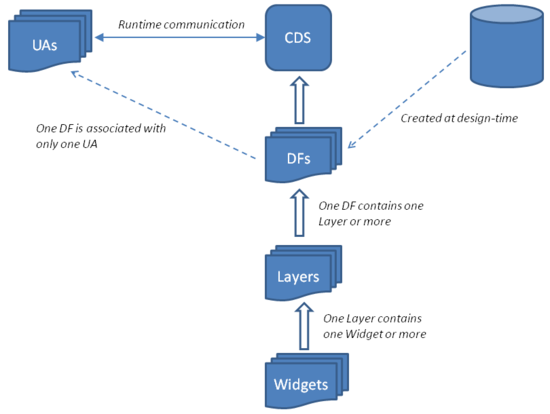
\includegraphics[width=0.6\linewidth]{img/ARINC_661_structure.png}
                \caption{ARINC 661 structure}
            \end{figure}
        \subsubsection{GUI Definition}
            Each DF binary file specifies the GUI definition for one User Application (UA) User interface. Several UA user interface trees can 
            be combined to constitute the CDS display definition. \\
            \vspace{3mm}
            A DF is composed of two parts : an optional symbol definition, and a widgets definition. The widget library is similar to Widgets 
            used in computing. There are Containers, Lists, ScrollPanes, Buttons, Menus, Labels, EditBoxes, etc... \\
            \vspace{3mm}
            Although the DF File is binary, the standard has also defined an associated XML definition, which is easier to manipulate in tools.
    \subsection{User Application}
        The UA contains the logic for each CDS. There are three generic CDSs are developed:
        \begin{itemize}
            \item Primary Flight Display (PFD)
            \item Fuel page
            \item Radio page
        \end{itemize}
        Each CDS is controlled by a UA. The main task for each UA is to update the widget's paremeters by sending precisely defined 
        ARINC 661 messages to the CDS. The UA uses the simulator global variables such as speed, altitude, heading, etc., through a 
        tailored simulator interface called SimIF, to build the message for the CDS. SimIF is a library that enables the UA to write 
        and read simulator variables to and from the shared memory, which contains the global variables that the simulator needs to 
        run its applications, including the PFD, fuel and radio variables.
    \subsection{Cockpit Display System}
        The CDS is made up of a number of Layers controlled by one UA. In A661, a Layer is the highest entity of the CDS as seen by 
        the UA. From a CDS viewpoint, a Layer is a graphical entity related to the application within a window page. Layers are numbered 
        and can be connected to a SuperLayer. Each Layer contains several widgets that are displayed as objects. The SuperLayer links all 
        UA Layers for the flight deck together by a single CDS Layer. The SuperLayer also uses standard widgets, to define all of the 
        groupings of functional UA Layers that are needed to draw each display and uses connectors to reference those functional UA 
        Layers as shown in below figure.
        \begin{figure}[H]
            \centering
            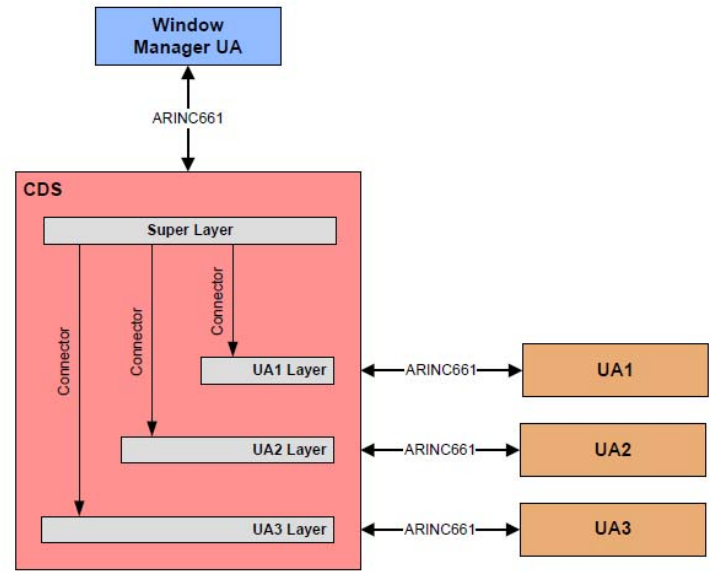
\includegraphics[width=0.6\linewidth]{img/SuperLayer.PNG}
            \caption{Super layer}
        \end{figure}
        This figure shows a Display Unit that has a set of windows, and each window is subdivided in a number of layers, which are owned 
        by their respective UA.
        \begin{figure}[H]
            \centering
            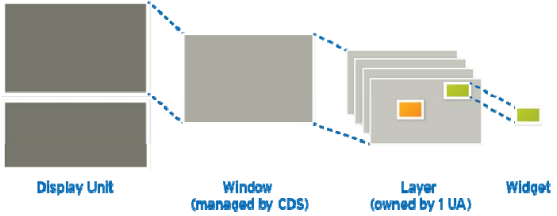
\includegraphics[width=0.6\linewidth]{img/window-layer.PNG}
            \caption{Window \& Layer illustration}
        \end{figure}
    \subsection{Window Manager}
        The Window Manager’s primary task is to manage all the logical display of each CDS page as well as the page’s selection interface, 
        for the user to control \textbf{(CDS+UA)}.


\section{Interface panels power and requirements}
    \subsection{Simulation Interfacing Concepts}
        Figure shownws a typical power, lighting and interface signal requirements to drive an aircraft and simulated instruments/panels.
        \begin{figure}[H]
            \centering
            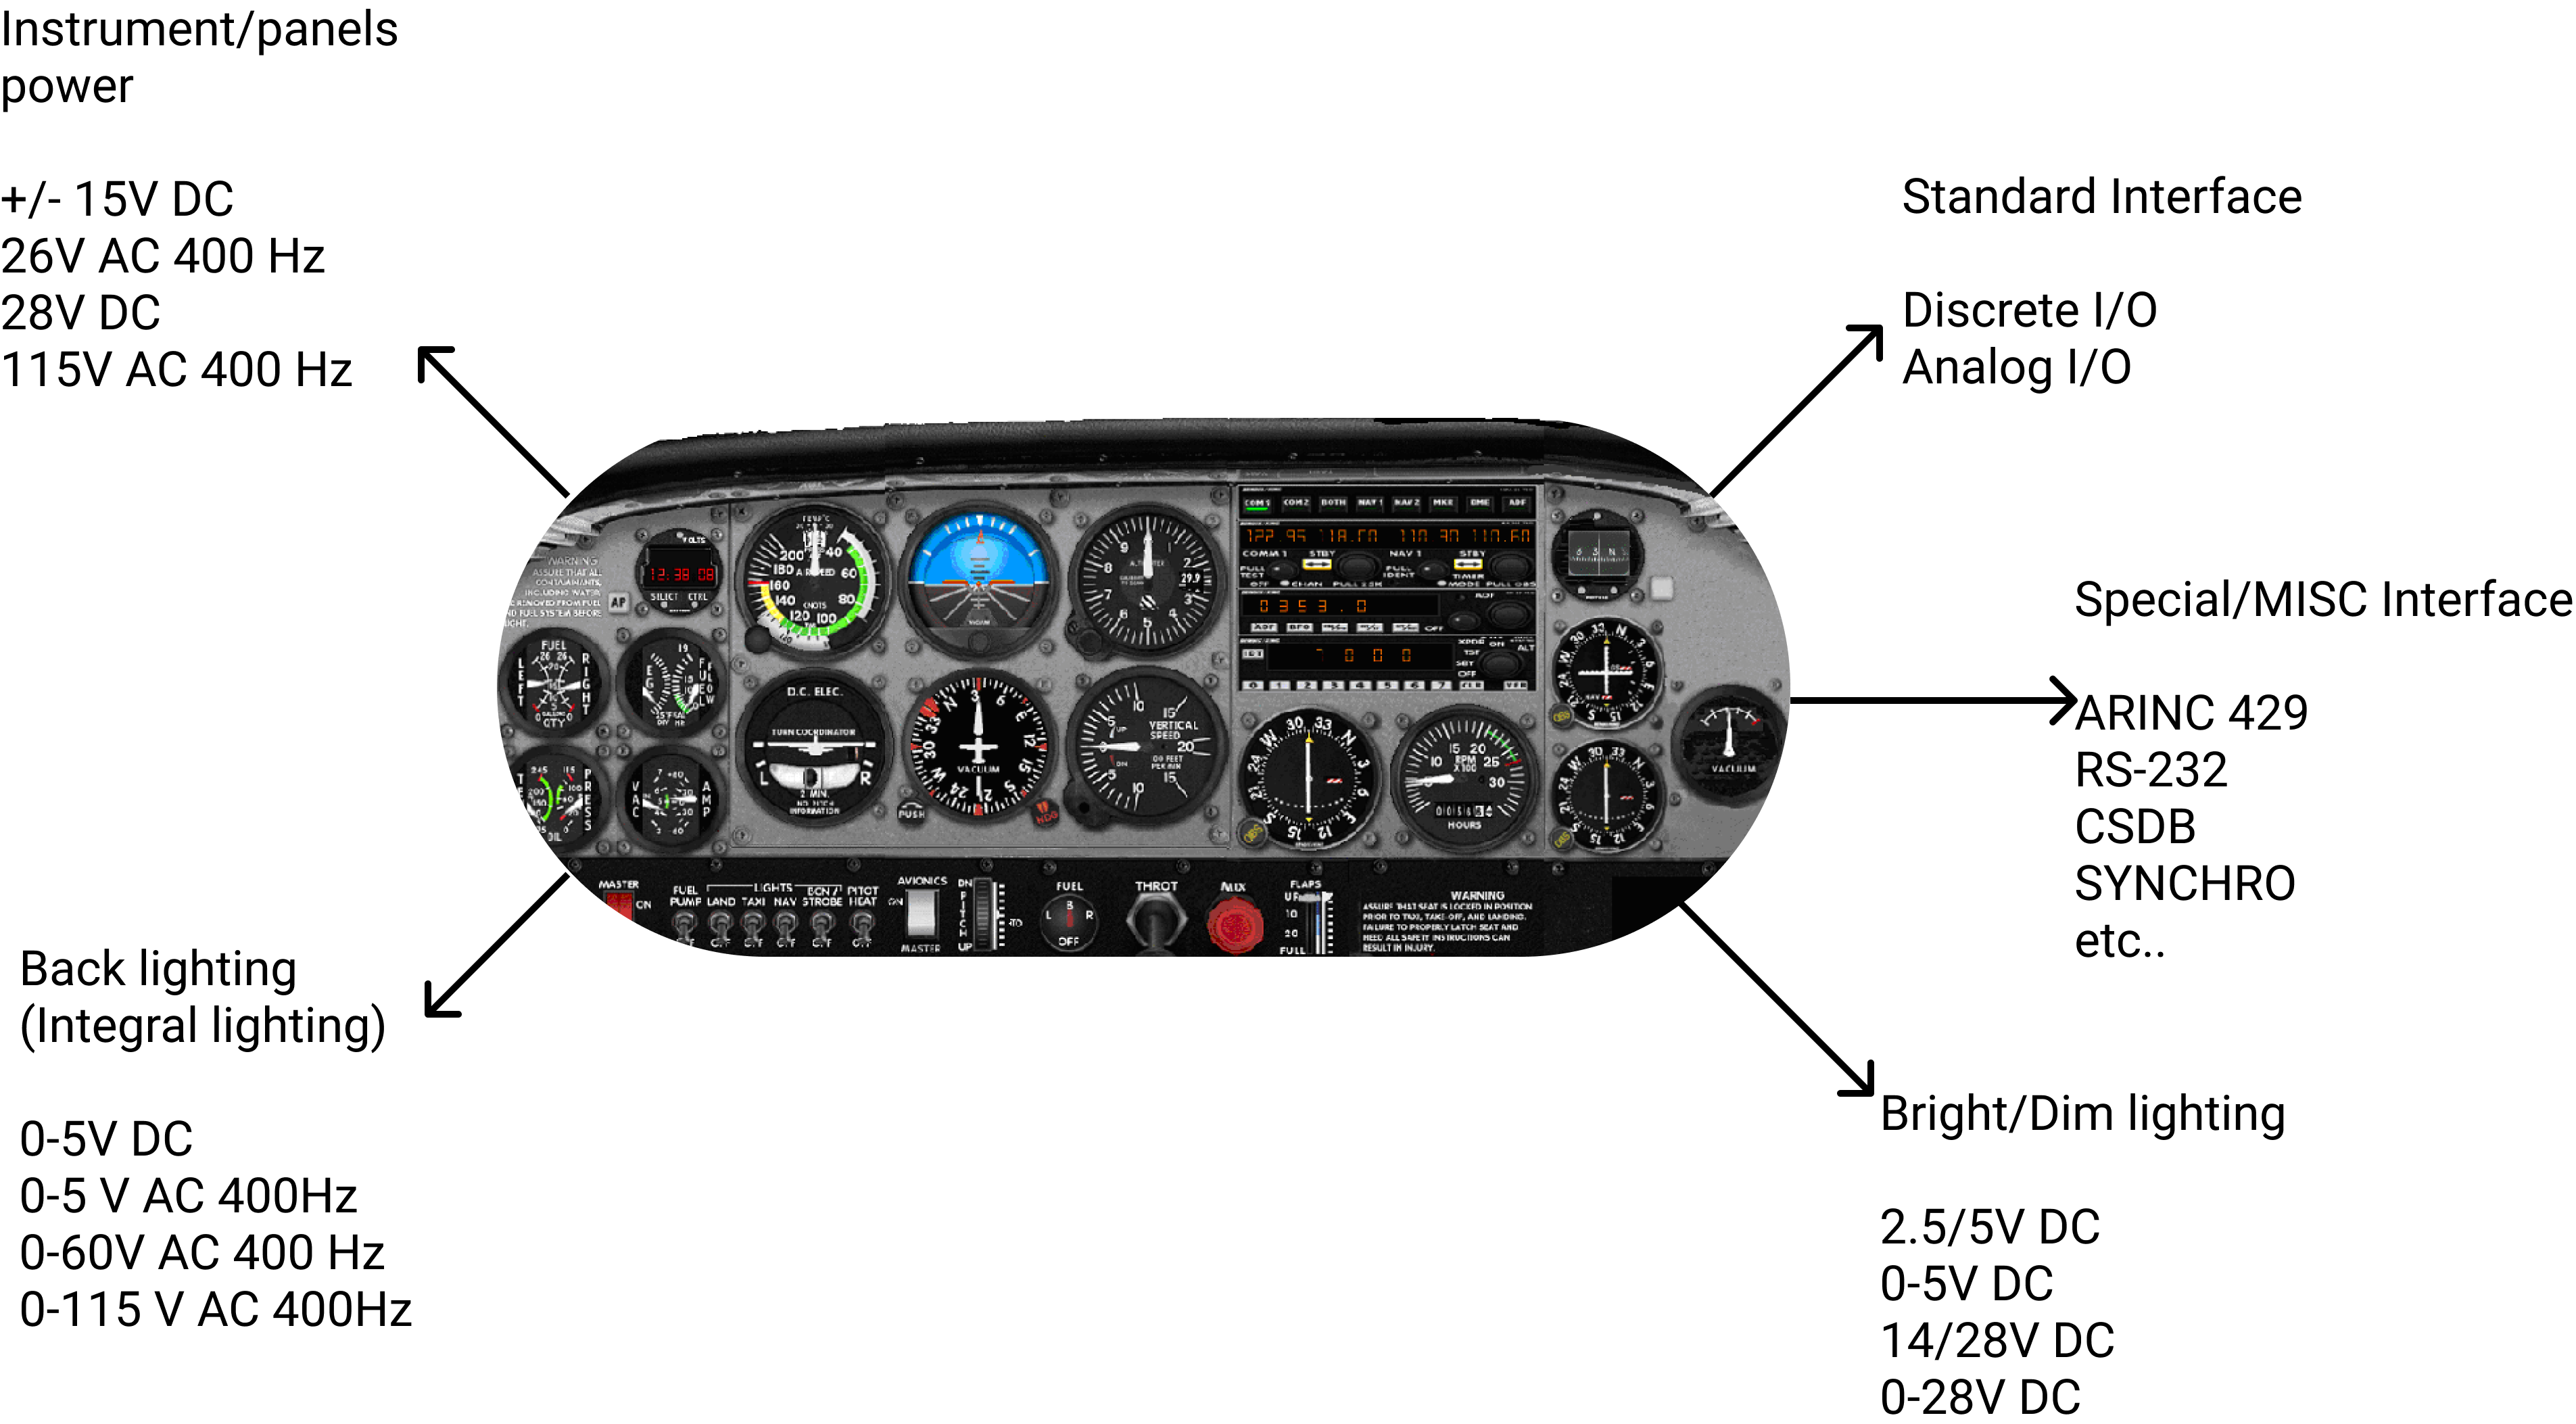
\includegraphics[width=0.6\linewidth]{img/Simulation.png}
            \caption{Aircraft panels power interface requirements}
        \end{figure}
        This figure is shown the Interface Systems Architecture.
        \begin{figure}[H]
            \centering
            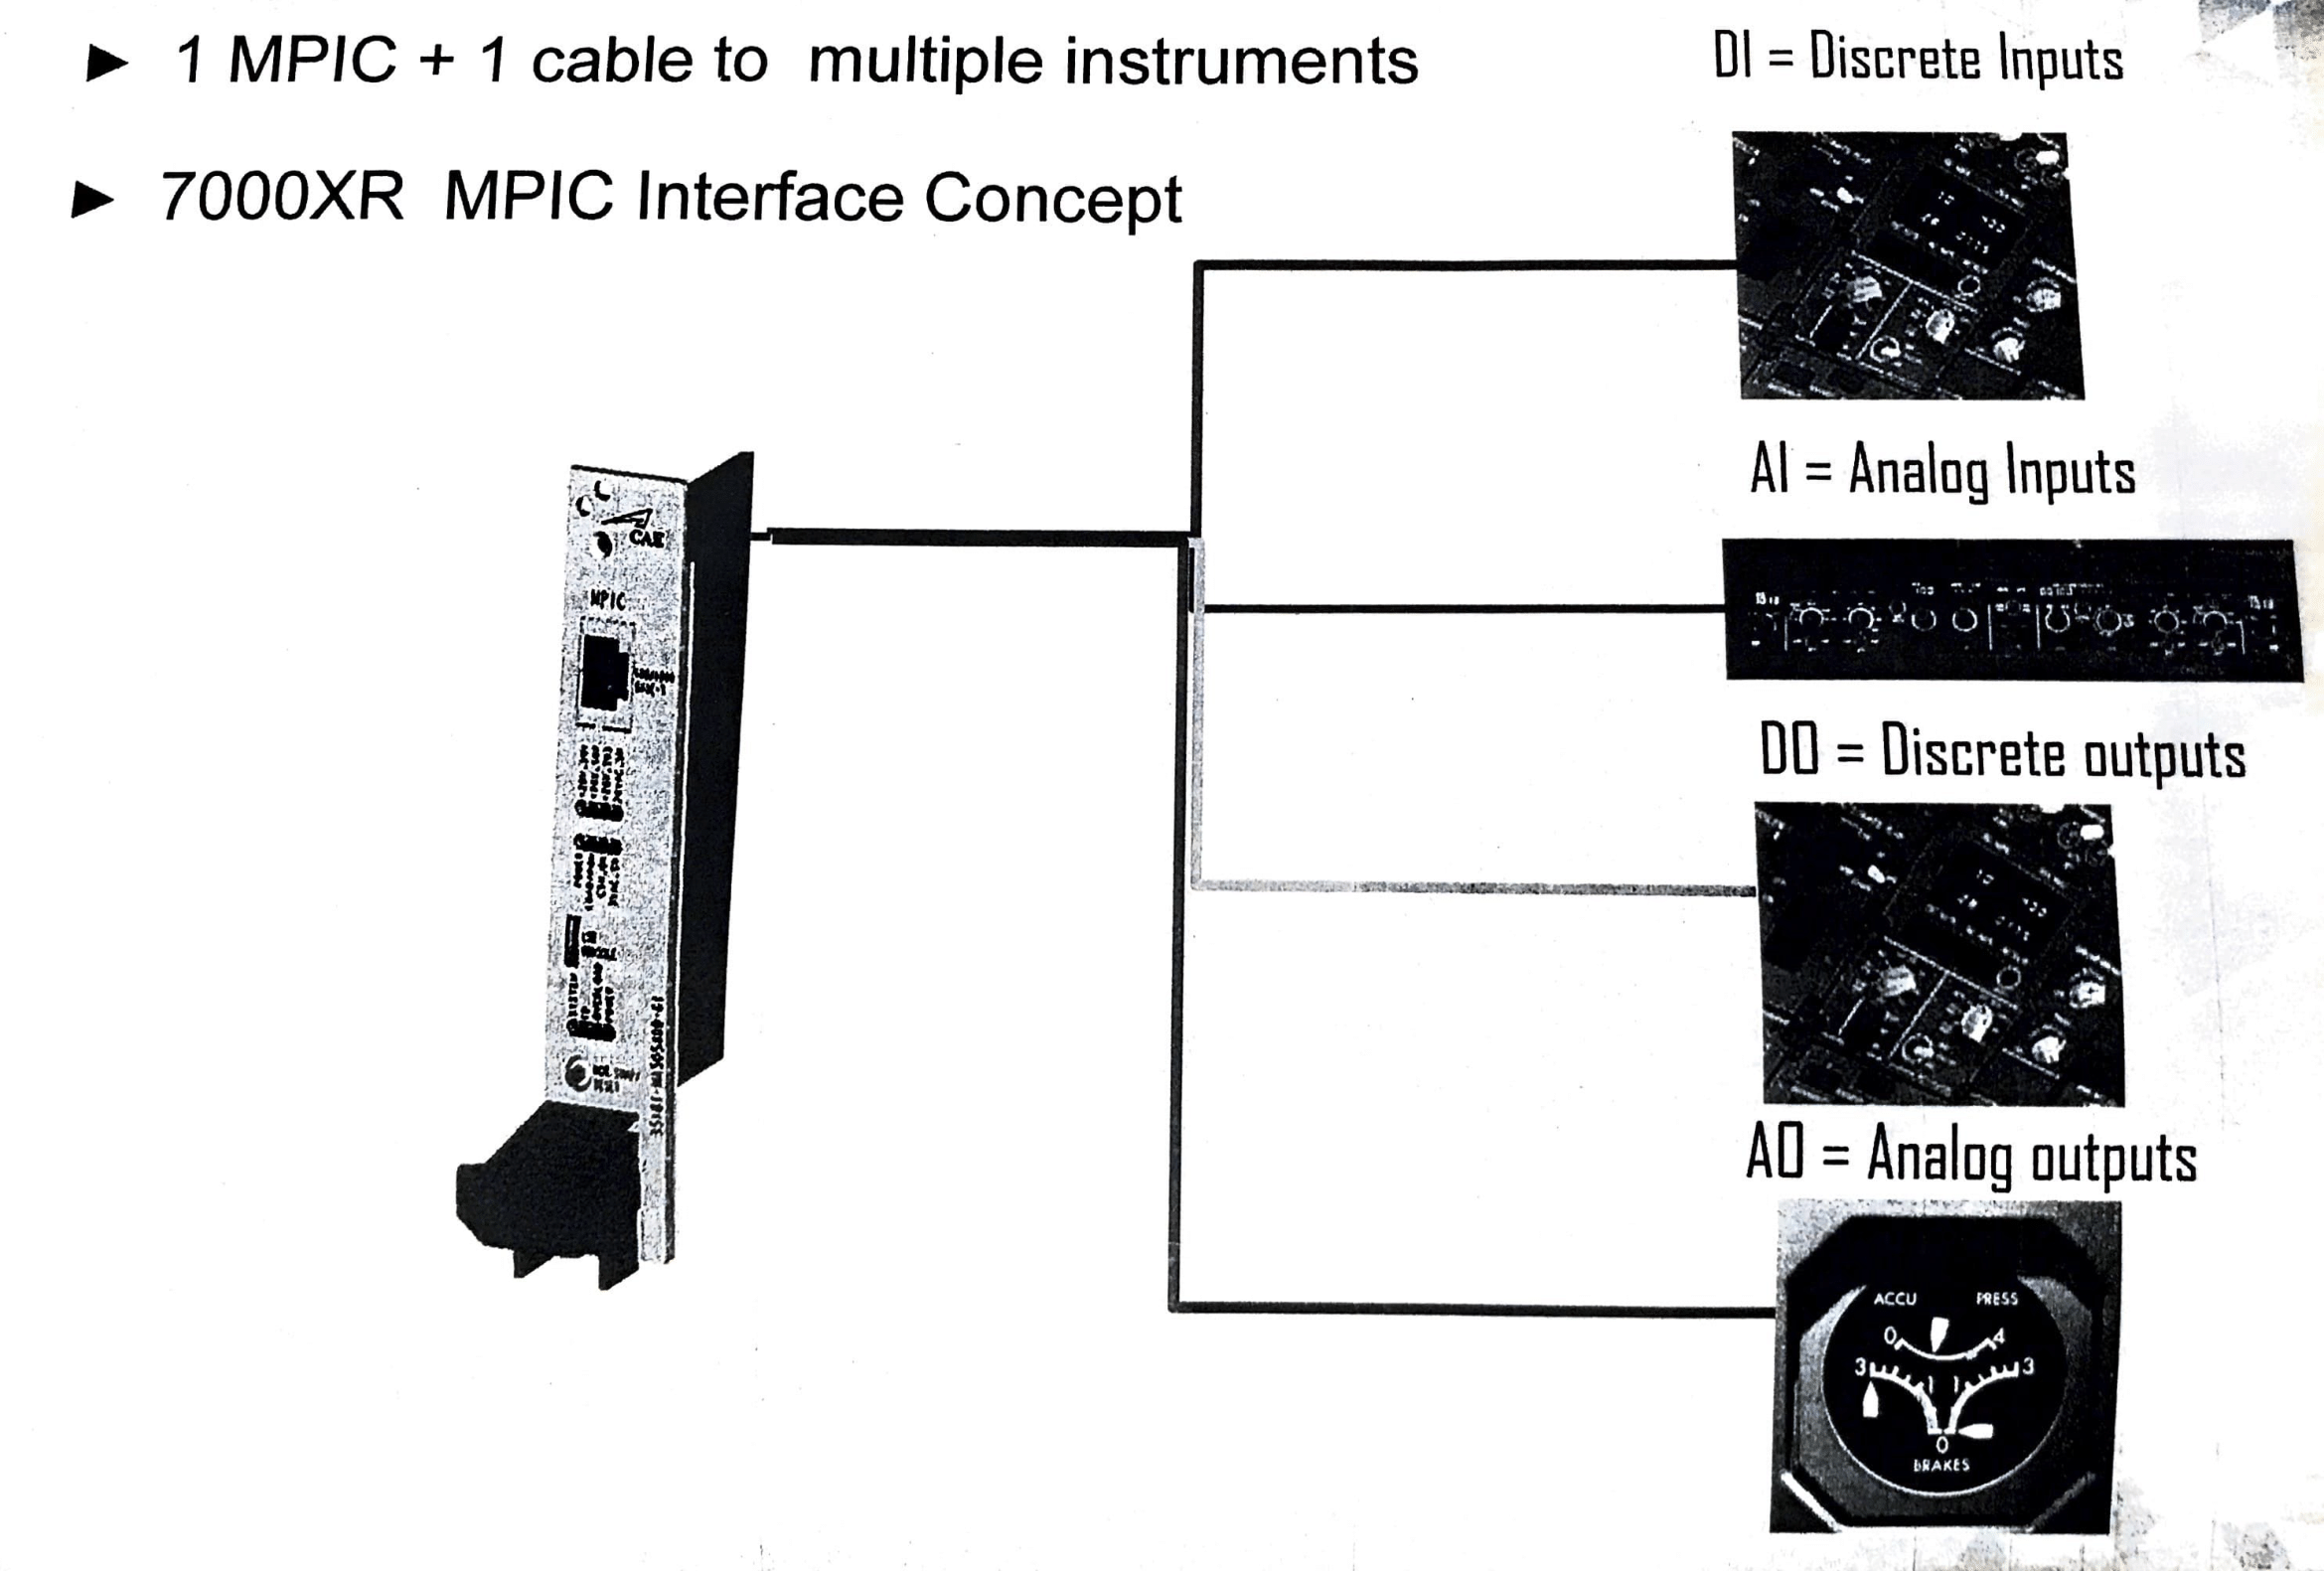
\includegraphics[width=0.6\linewidth]{img/image.png}
            \caption{Interface systems architecture}
        \end{figure}
        Figure below here shows an actual typical aircraft wiring diagram for a lighting functionality.
        \begin{itemize}
            \item A switch (SW) turns the lamp on/off;
            \item A circuit breaker (CB) powers the bus;
            \item Lamp could be for reading, map utility light or annunciator light switch.
        \end{itemize}
        \begin{figure}[H]
            \centering
            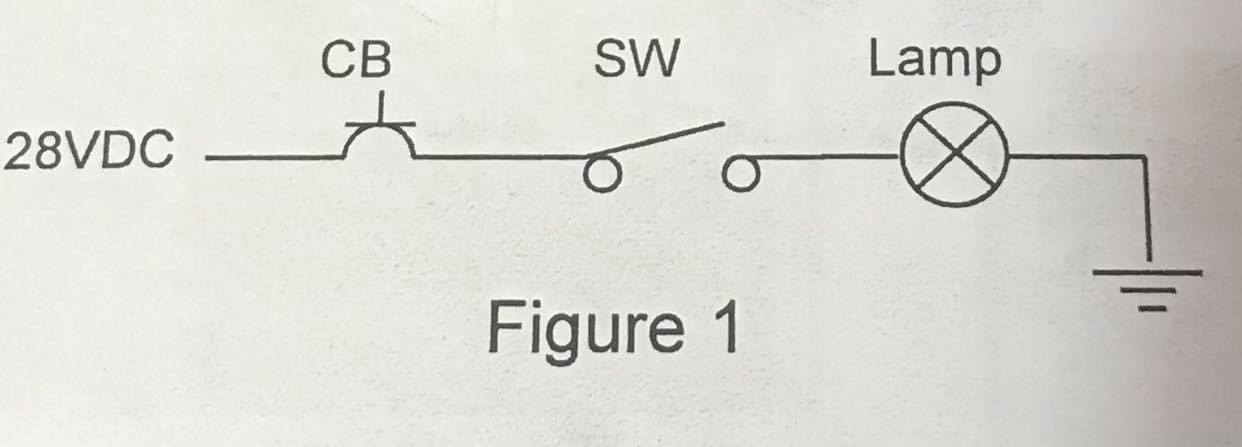
\includegraphics[width=0.6\linewidth]{img/figure1.jpg}
            \caption{Wiring diagram for lighting functionality}
        \end{figure}
        And the typical interface simulation wiring includes:
        \begin{itemize}
            \item The DIP GND on the MPIC senses the status (on/off) of a switch (SW) or a circuit breaker (simulated CB);
            \item DOP 28V on the MPIC turns the lamp on/off;
            \item Additional DOP 28V and DOP GND create a fault (mal-function) condition;
            \item Software simulation manages all the above actions and also occasionally broadcasts aircraft condition to other simulation 
            systems.
        \end{itemize}
        \begin{figure}[H]
            \centering
            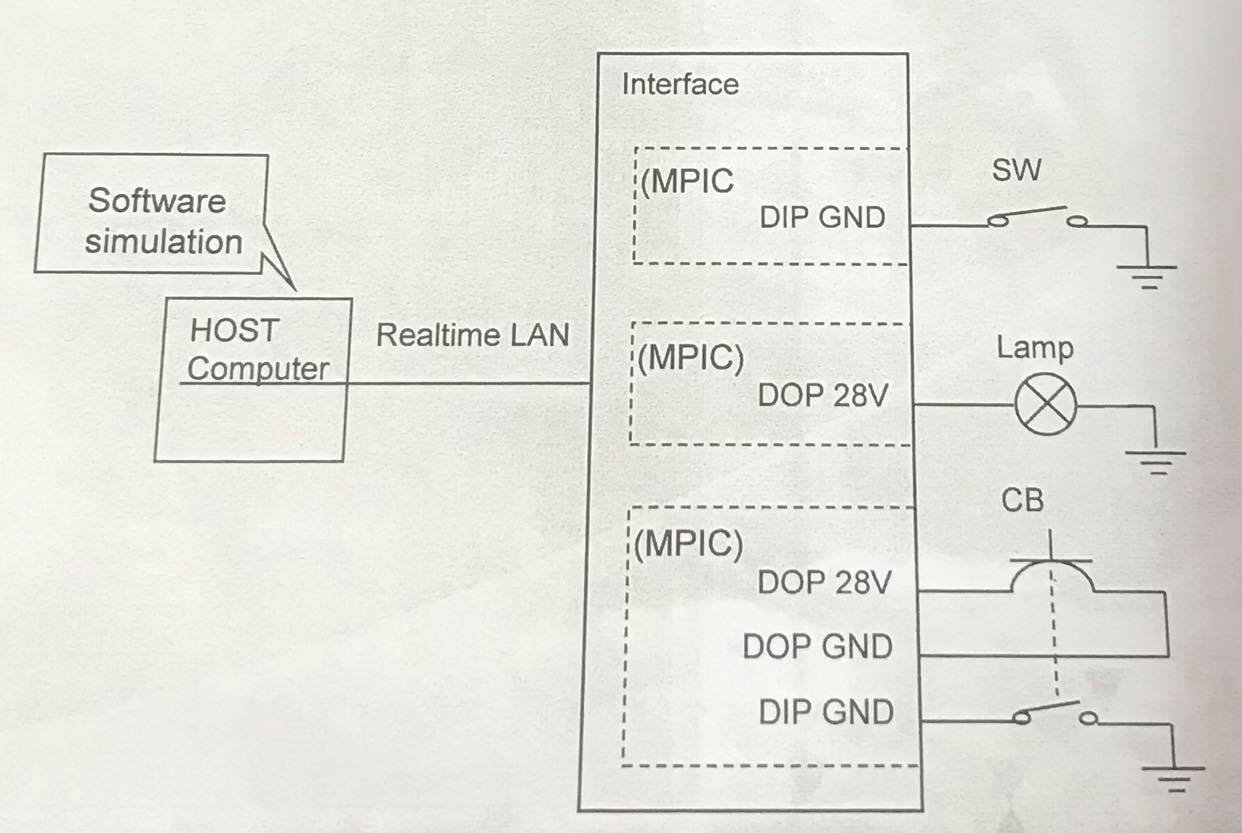
\includegraphics[width=0.6\linewidth]{img/figure2.jpg}
            \caption{Interface simulation wiring}
        \end{figure}
    \subsection{Major Components}
        \begin{figure}[H]
            \centering
            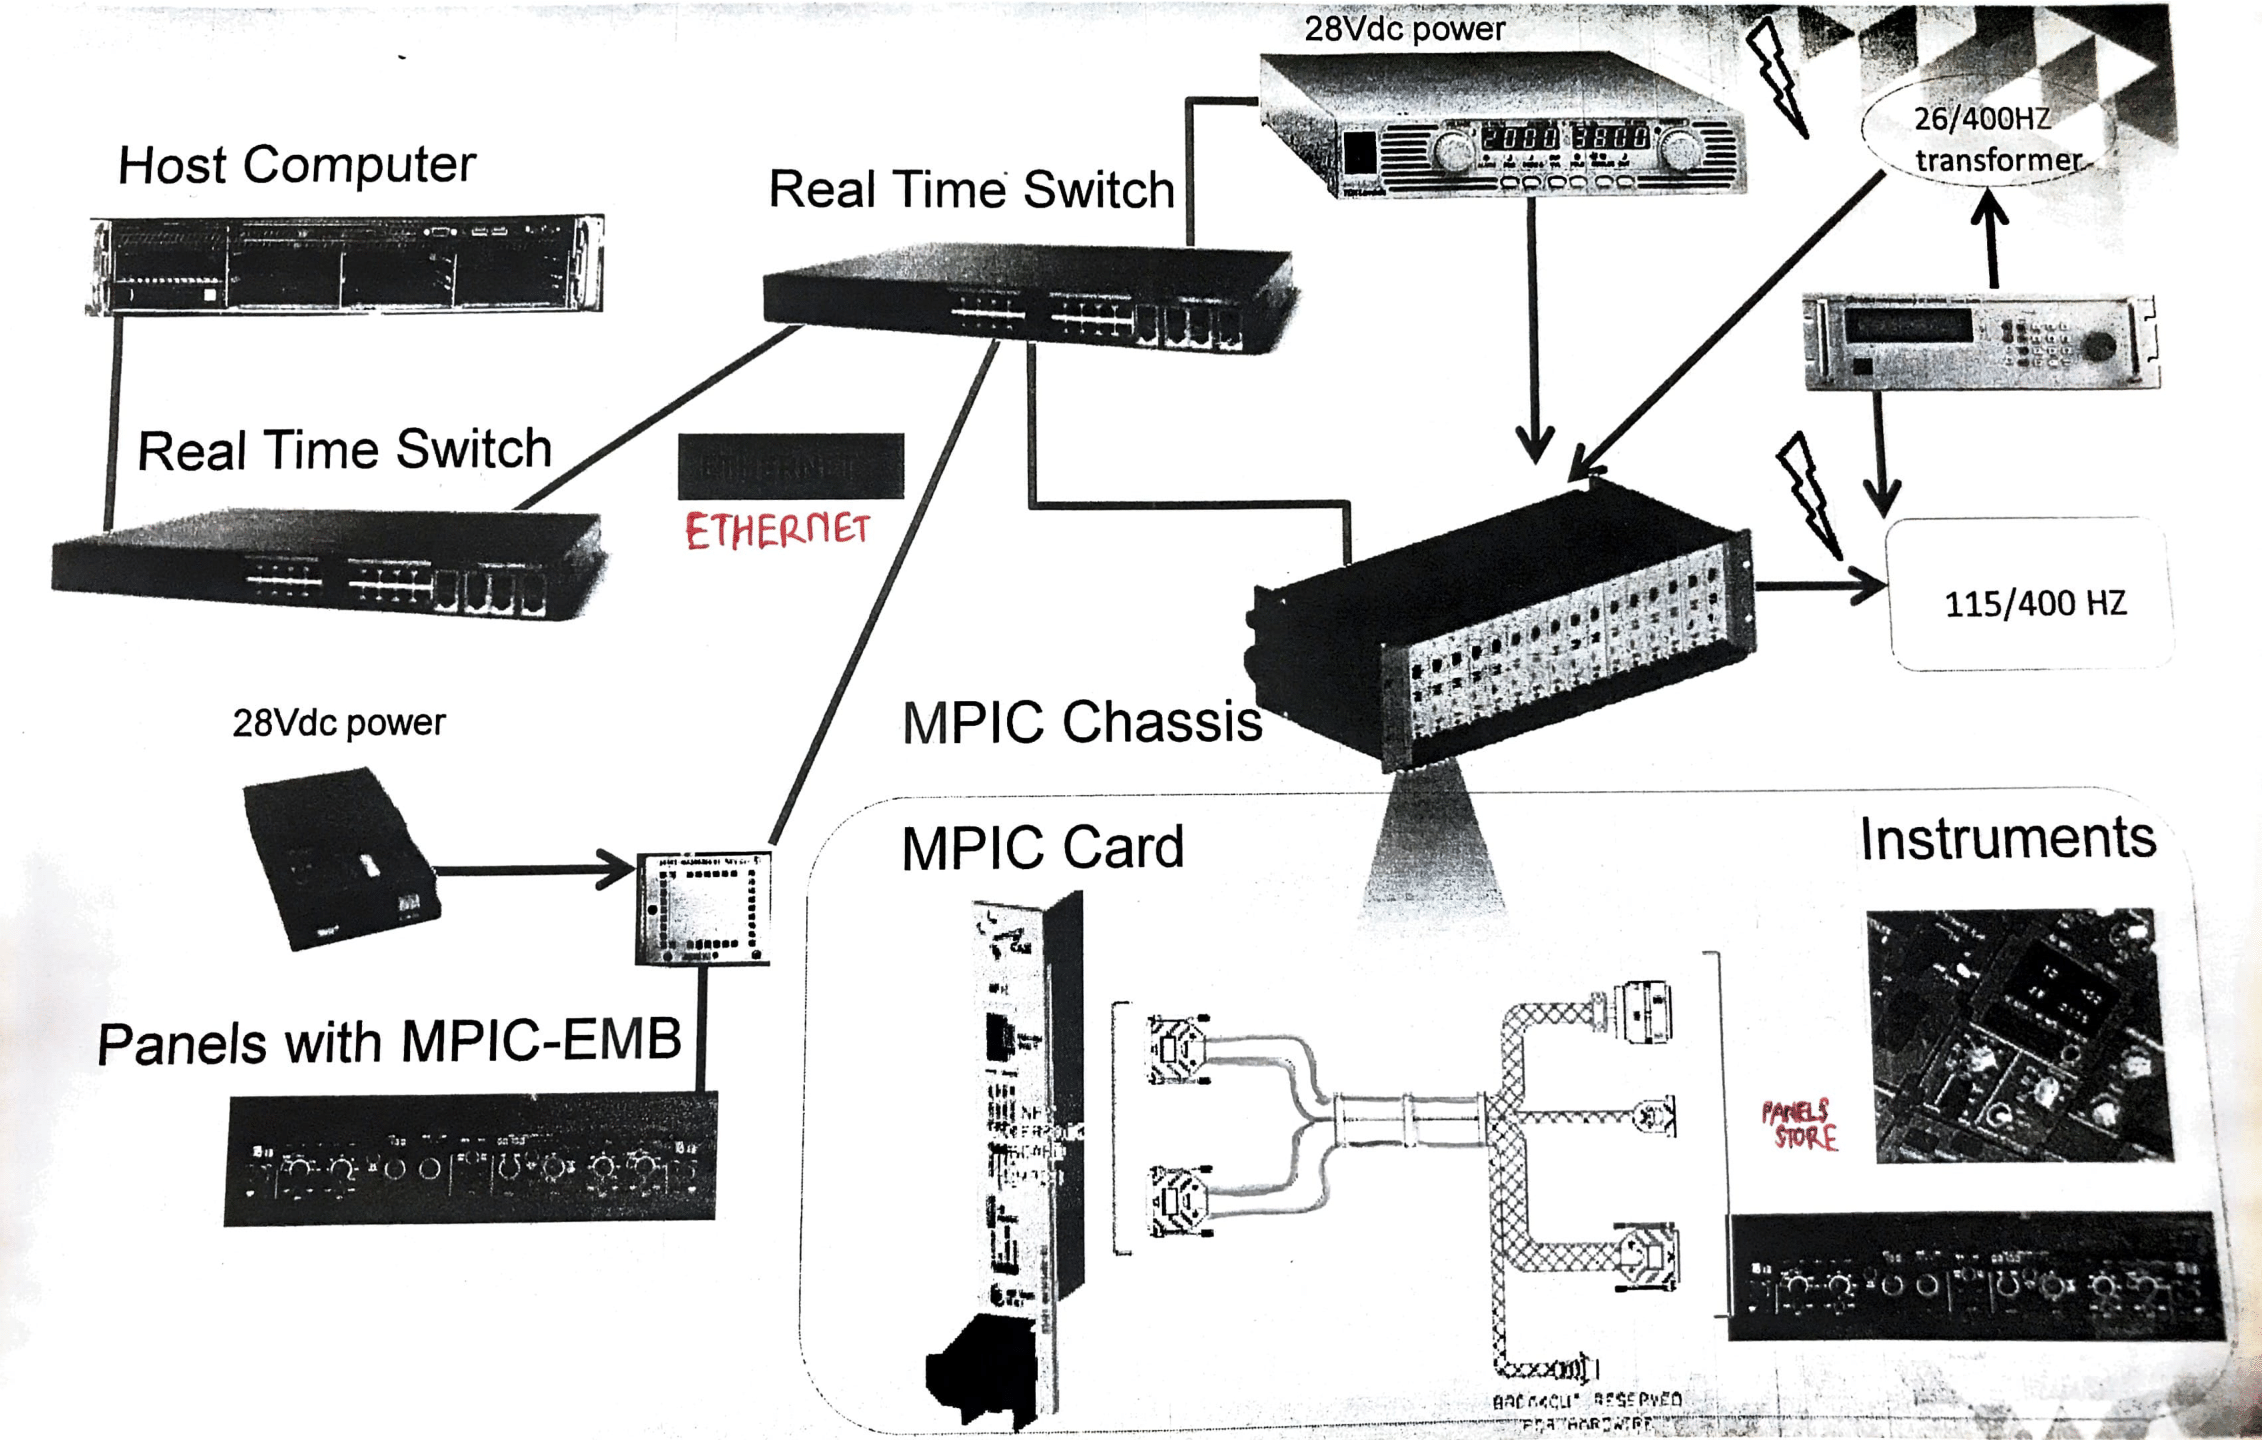
\includegraphics[width=0.6\linewidth]{img/require-component.png}
            \caption{Interface systems architecture}
        \end{figure}
        \begin{figure}[H]
            \centering
            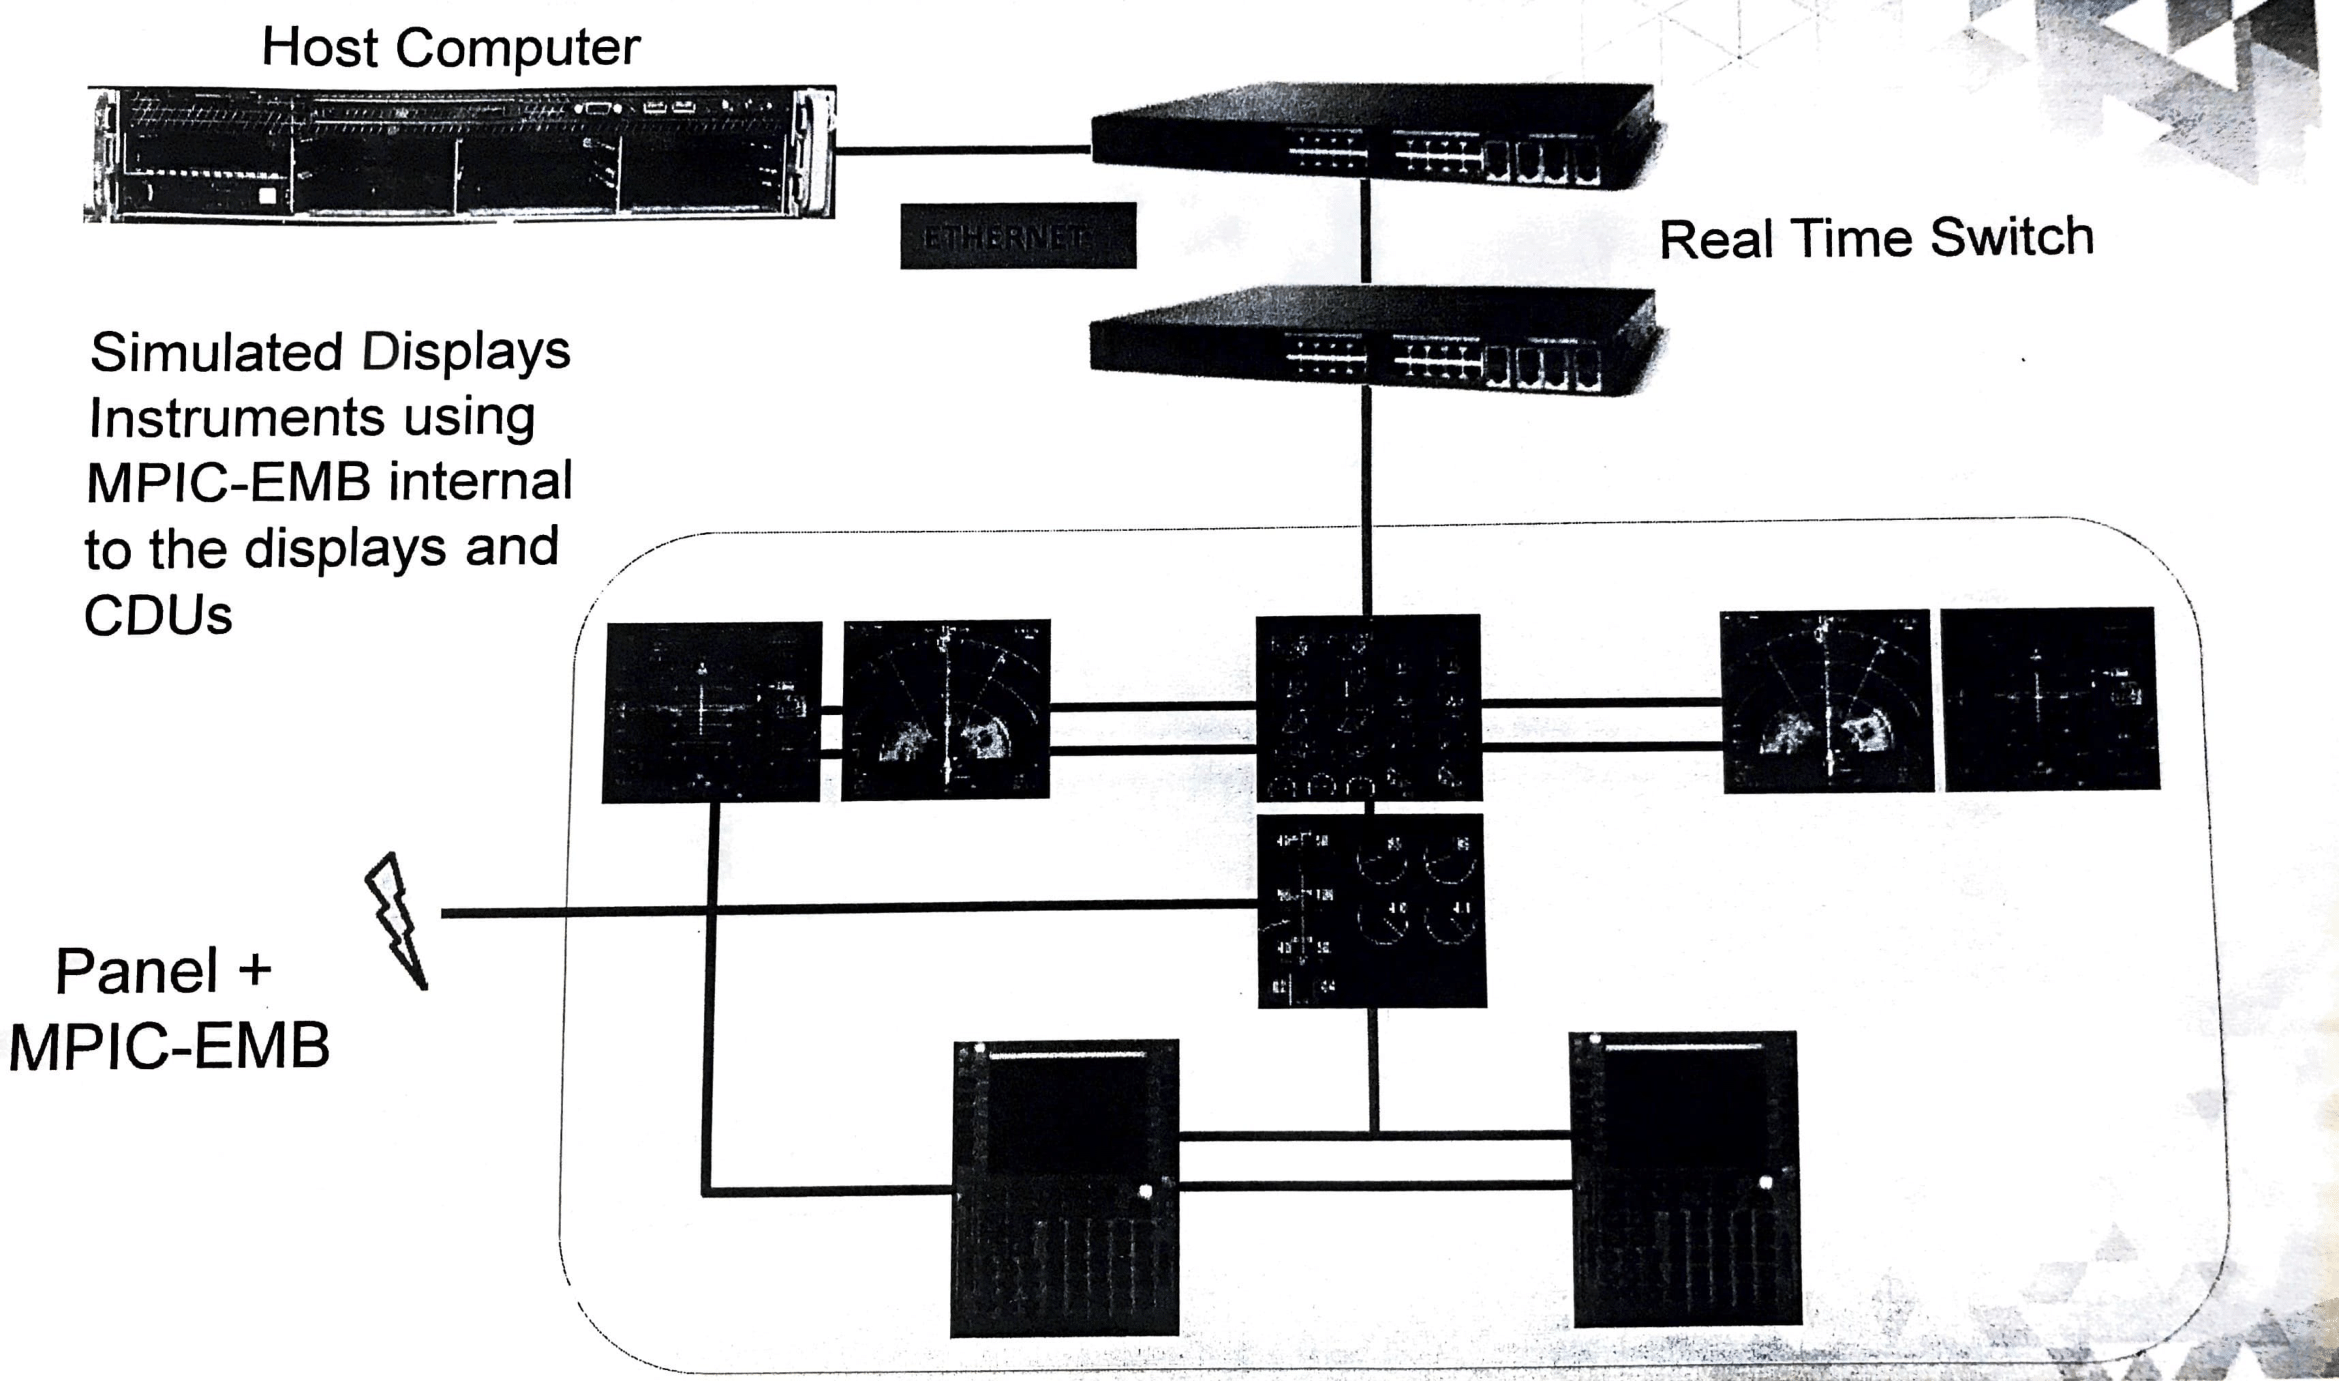
\includegraphics[width=0.6\linewidth]{img/Simulated-Display.png}
            \caption{Simulated displays instruments}
        \end{figure}
    \subsection{Network Architecture}
        \begin{figure}[H]
            \centering
            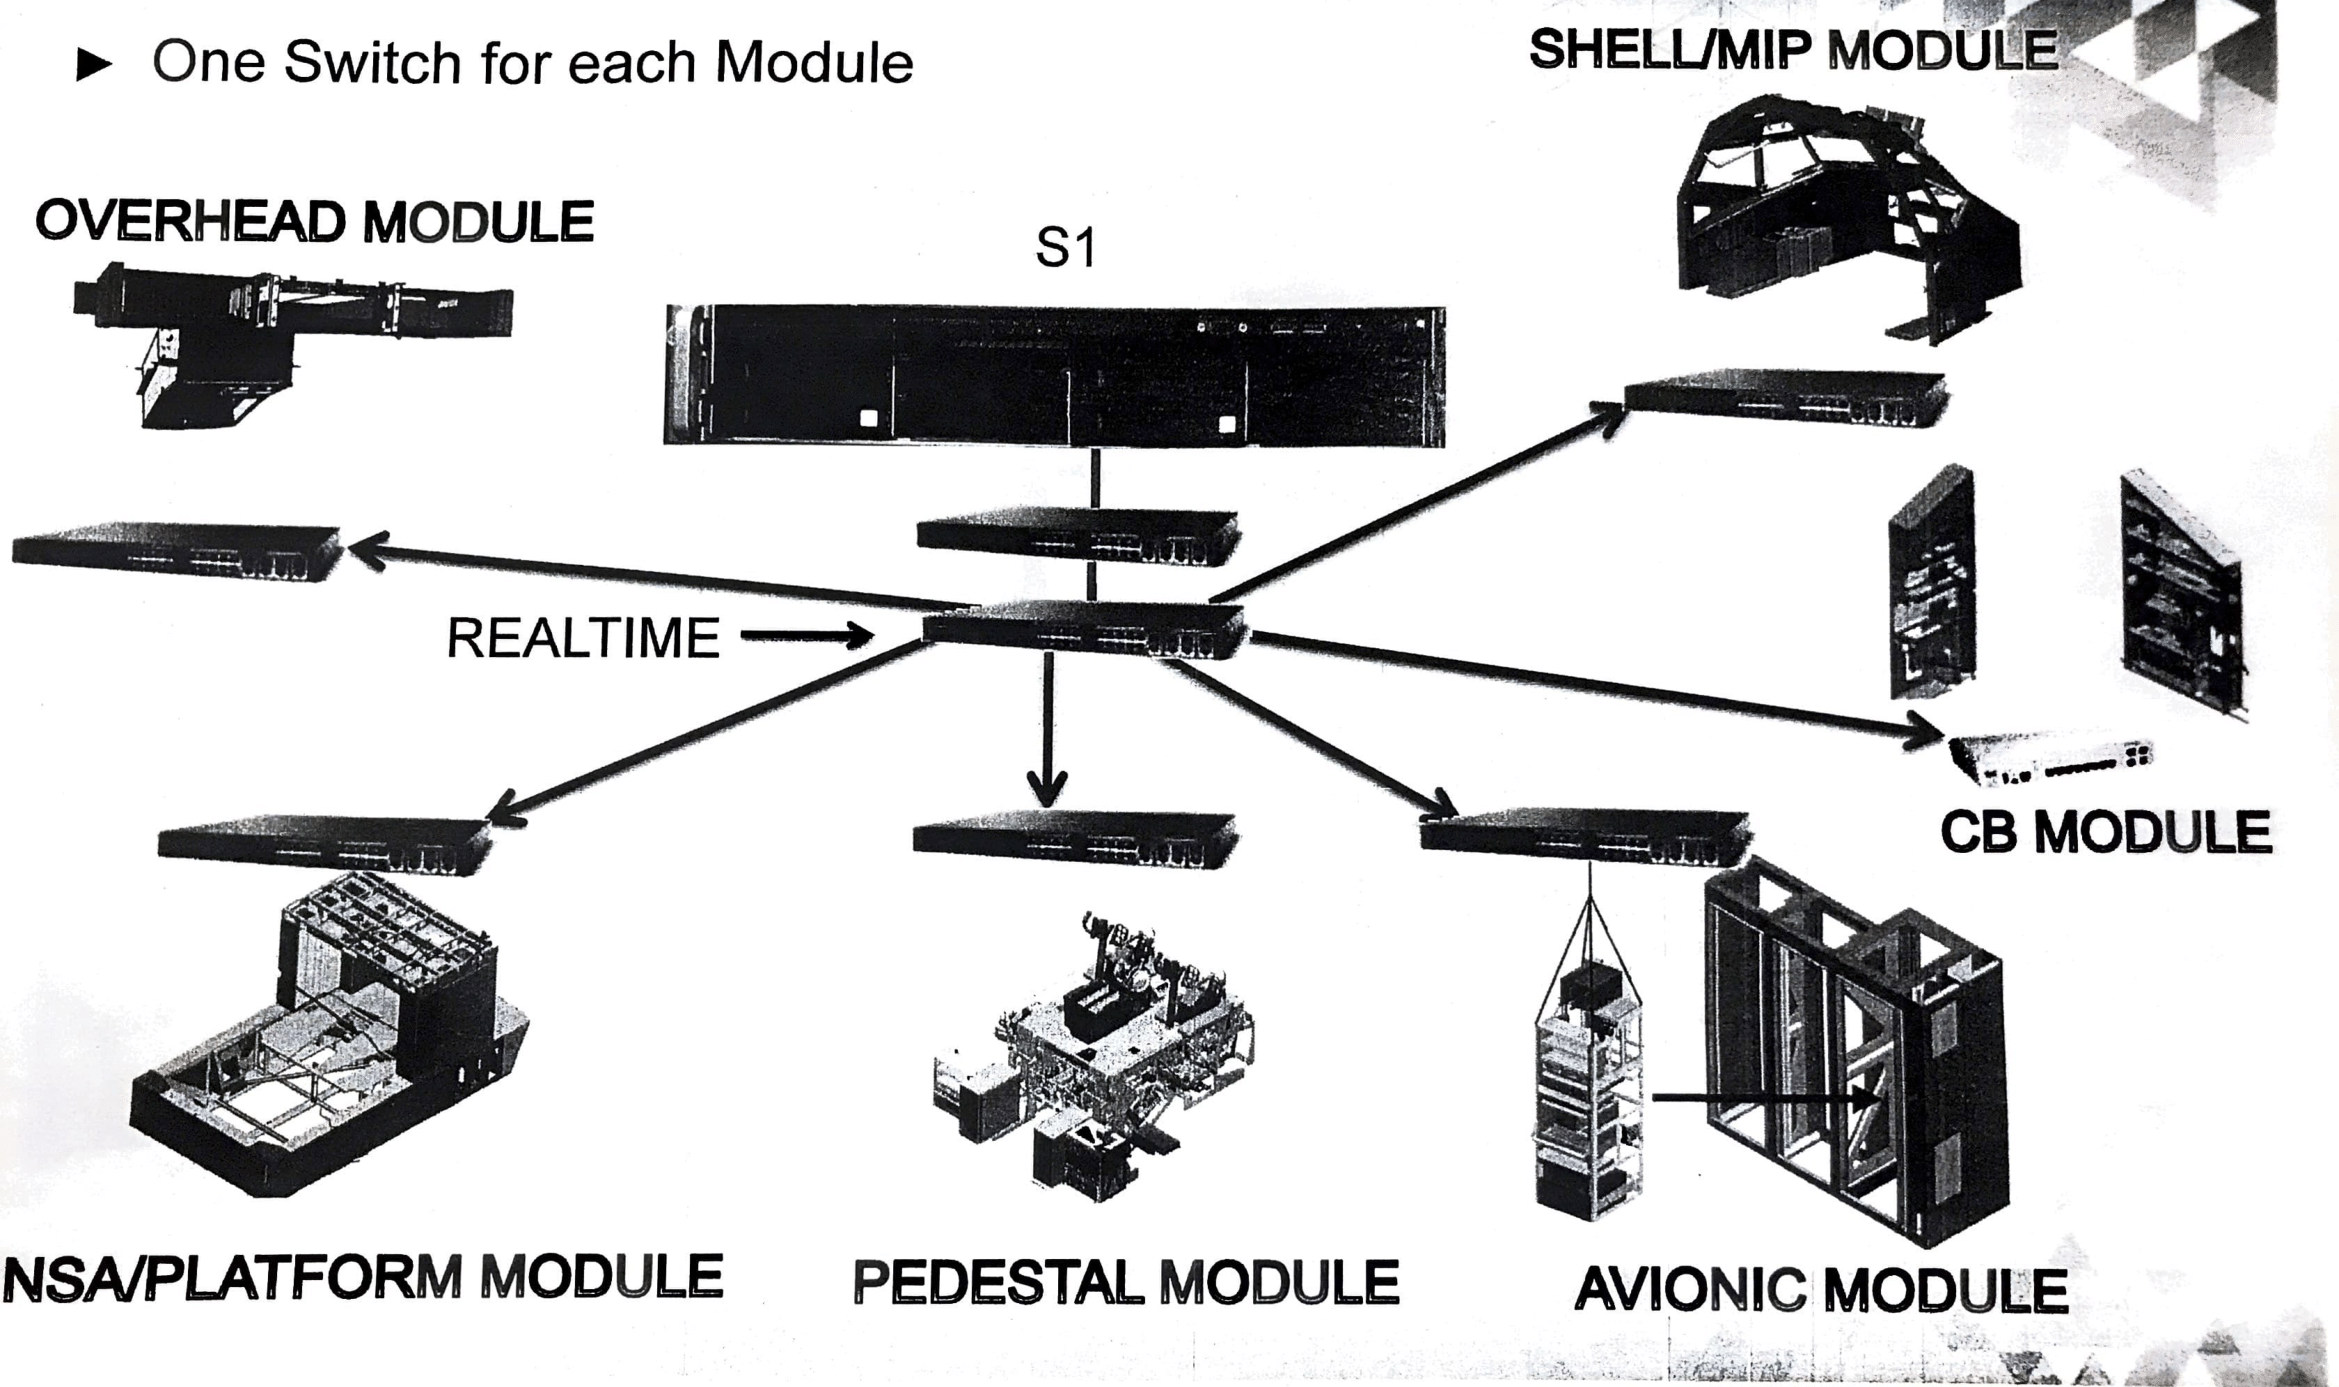
\includegraphics[width=0.6\linewidth]{img/network.png}
            \caption{Network modules}
        \end{figure}
        \subsubsection{Module Level}
            \begin{itemize}
                \item MPIC chassis is composed of 16 MPIC slots, each divided in groups of 4;
                \item Each group of 4 uses the same Ethernet cable;
                \item Each MPIC-EMB has its own cable;
                \item An Ethernet cable part of a group of 4 can be plugged into any card in that specific group.
            \end{itemize}
            \begin{figure}
                \centering
                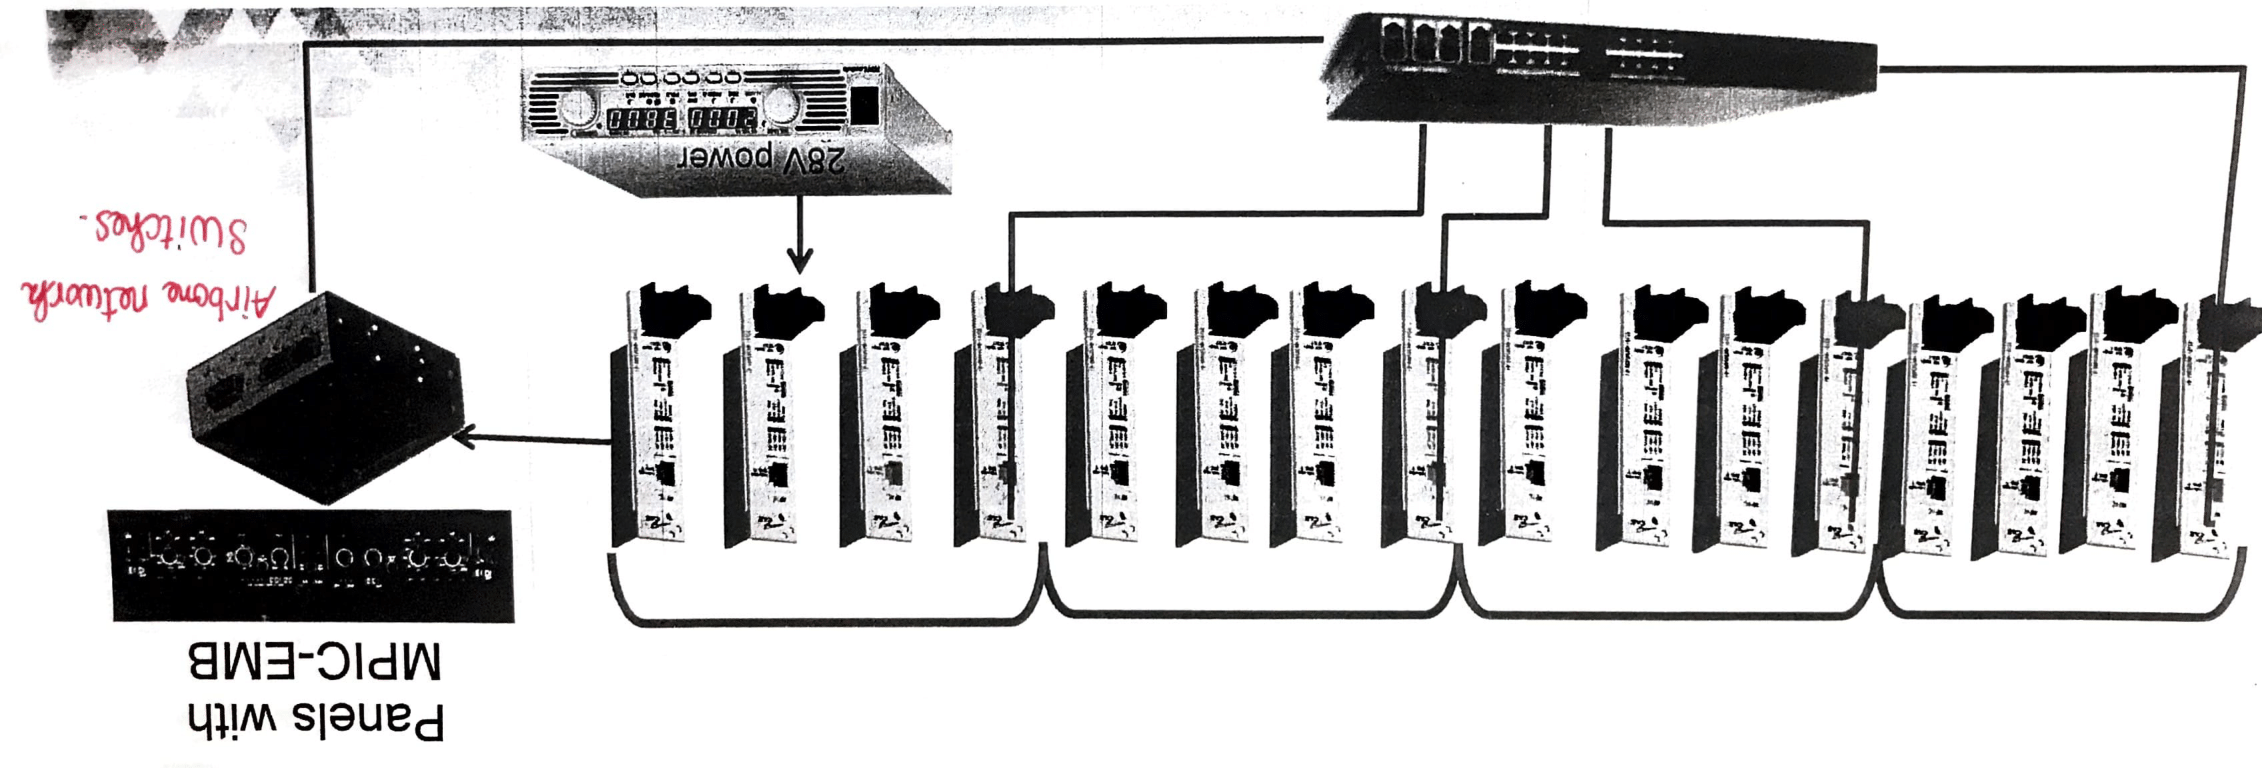
\includegraphics[width=0.6\linewidth]{img/Module-level.png}
                \caption{Module level network}
            \end{figure}
    \subsection{Communication Paths}
        Interface cards are connected to the Real time LAN. \\ 
        \vspace{3mm}
        Real time LAN is extended on the backplane.
        \begin{figure}[H]
            \centering
            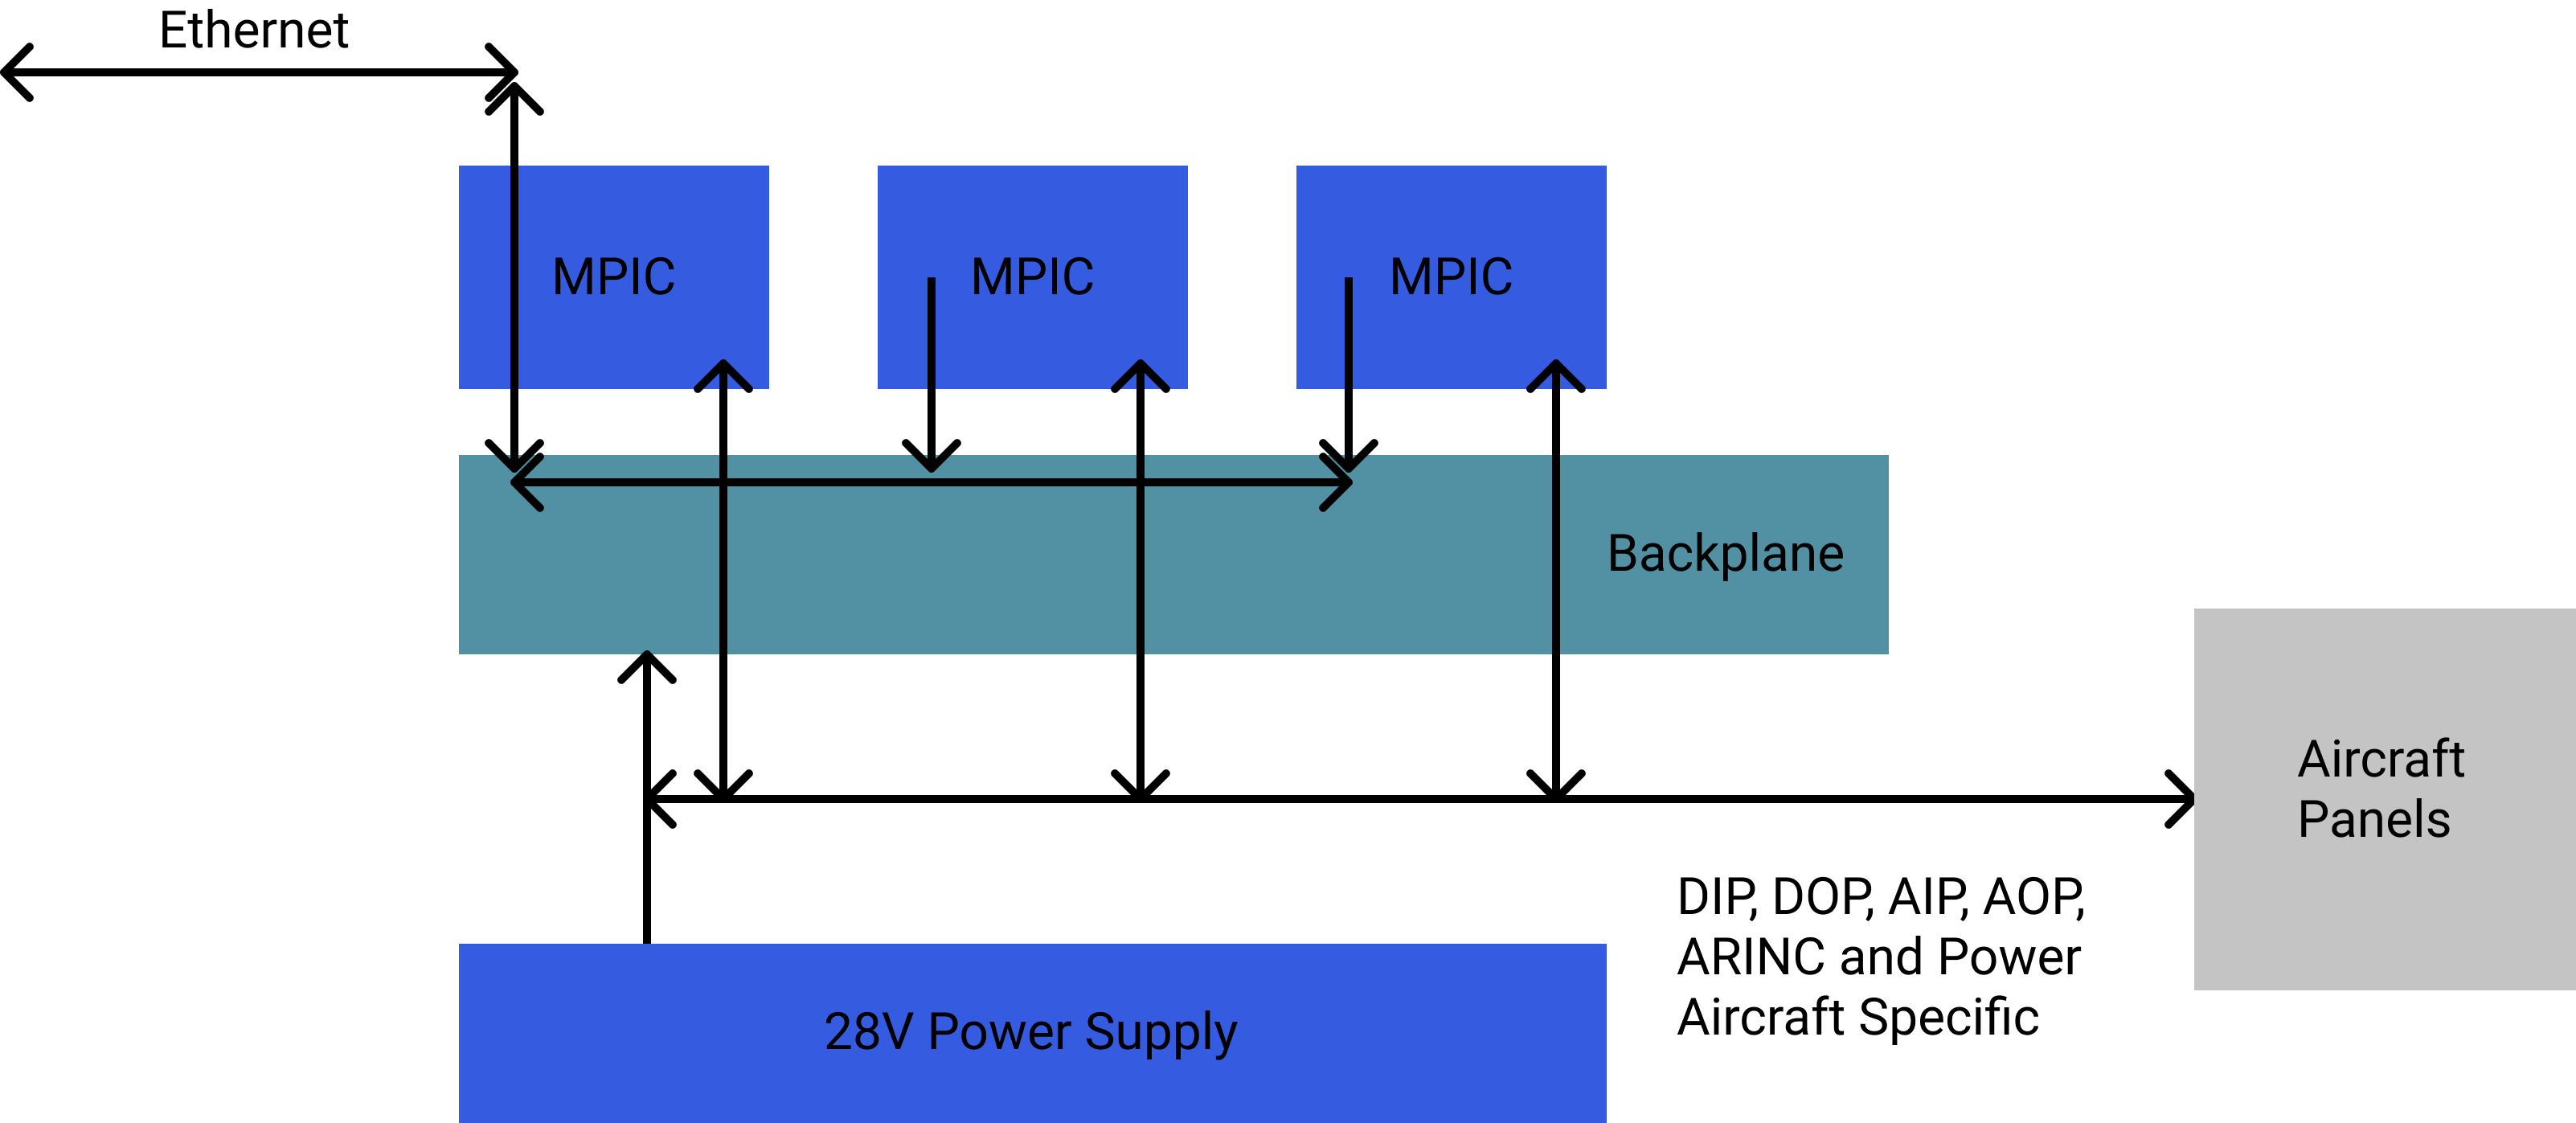
\includegraphics[width=0.6\linewidth]{img/communication path.png}
            \caption{Backplane}
        \end{figure}
    \subsection{Simulator Power Distribution}
        \begin{figure}[H]
            \centering
            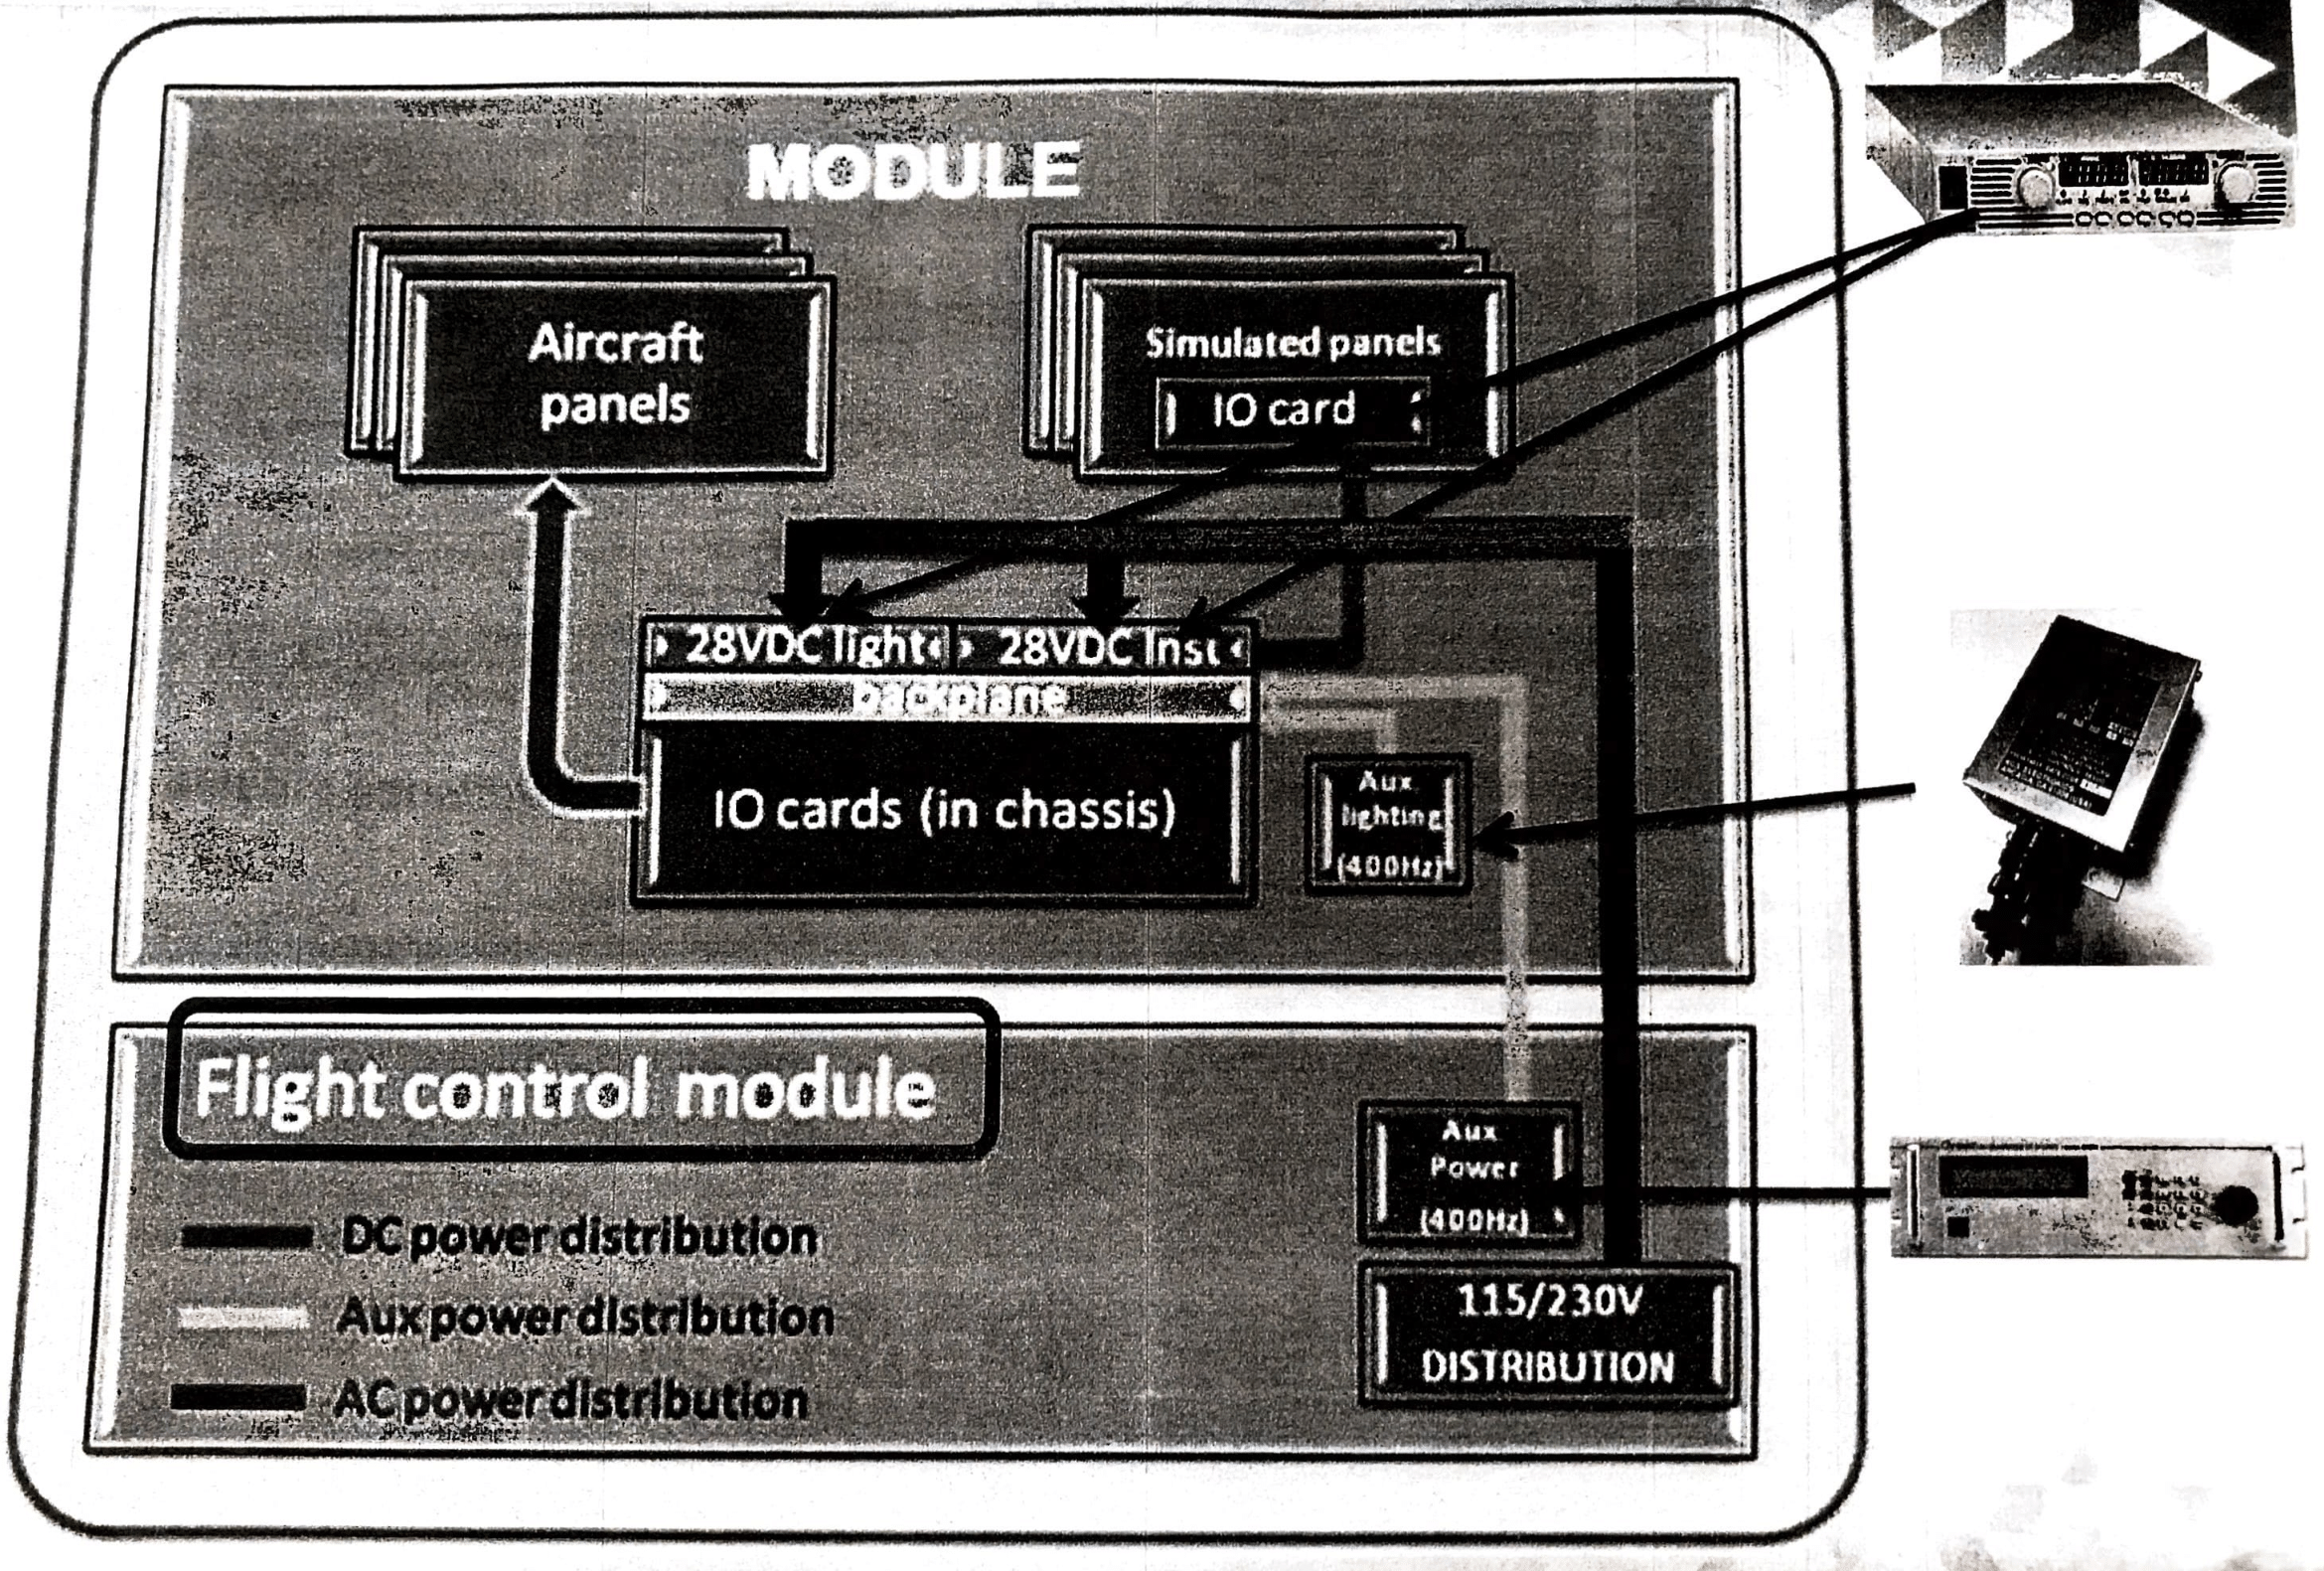
\includegraphics[width=0.6\linewidth]{img/flight-control.png}
            \caption{Flight control module}
        \end{figure}
        \begin{figure}[H]
            \centering
            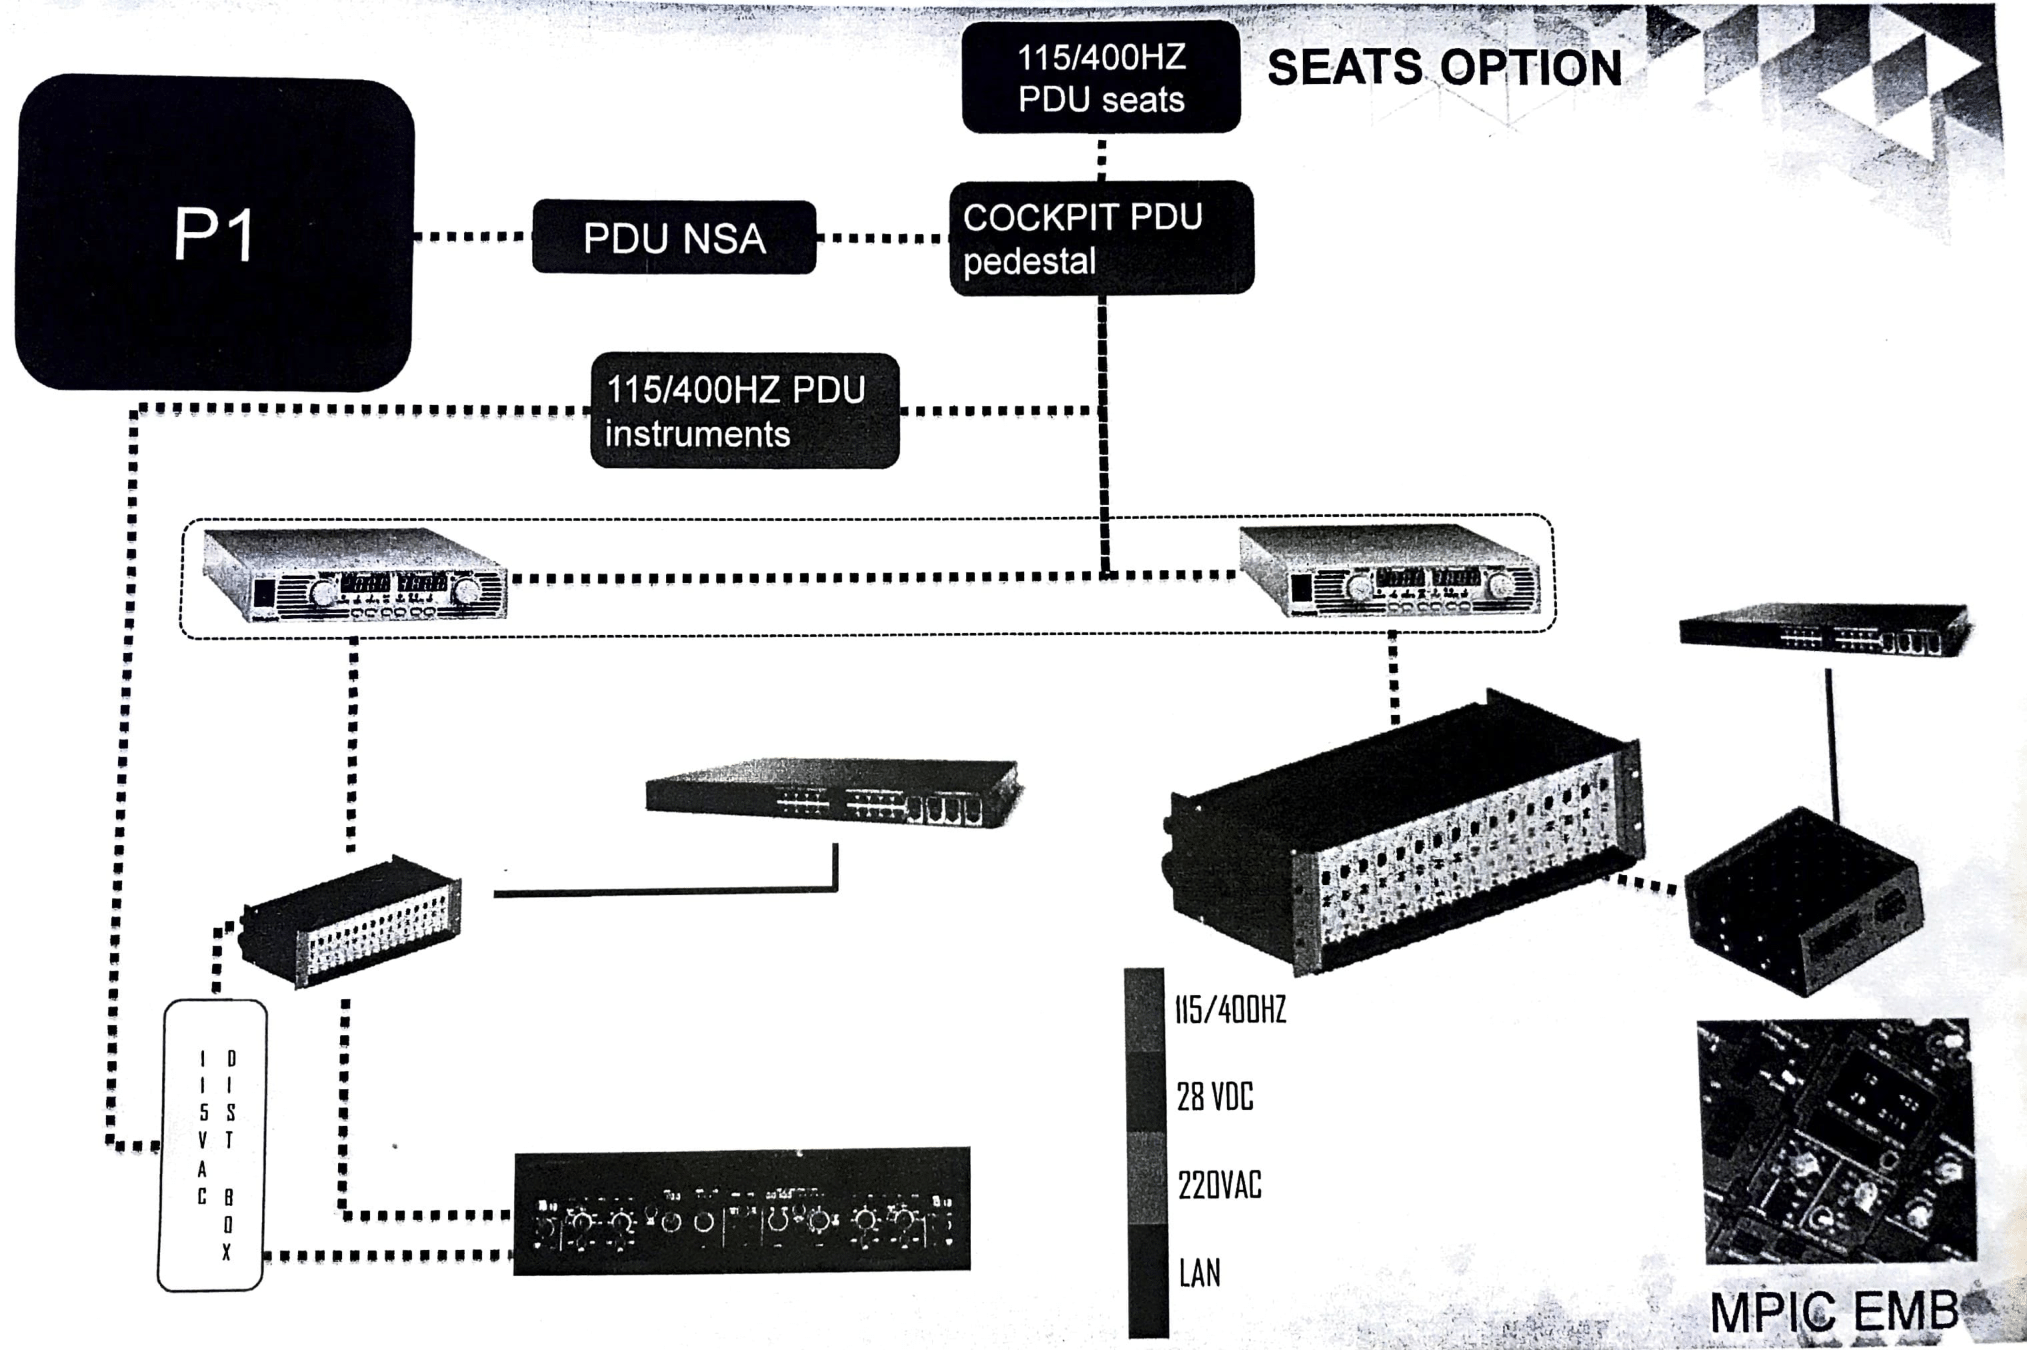
\includegraphics[width=0.6\linewidth]{img/seat-option.png}
            \caption{Seats option}
        \end{figure}
    

\section{Generic CDS Testing}
    Three generic CDSs have been initially created and tested on the CAE-MPIC. The development and tests conducted of those 
    CDSs and their related UAs helped understand the specificities of ARINC 661. Furthermore, it allowed to observe some 
    performance limitations and to determine the relevant benchmarking tests that must be further conducted. The CDSs designed 
    for the preliminary testing are very simple; the goal being the familiarization with the A661 standard.
    \subsection{PFD}
        The PFD is a non-interactive CDS. The widget positions are determined by the commands sent by the UA. The UA
        treats data received from the simulator. This new A661 PFD displays the same information as the simulator’s PFD. 
        This figure down here shows the PFD designed for the Benchmarking phase. 
        \begin{figure}[H]
            \centering
            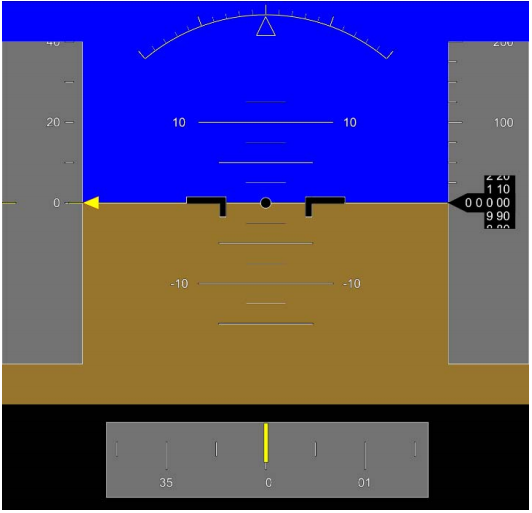
\includegraphics[width=0.6\linewidth]{img/PFD.PNG}
            \caption{Primary Flight Display (PFD)}
        \end{figure}
    \subsection{Fuel and Radio Page}
        Fuel and radio pages are interactive CDSs. Data is transmitted by the simulator to the UA that commands the appropriate W. 
        The user has the ability to send commands to the simulator. The selection is done with interactive A661\_TOGGLE\_BUTTON widgets. 
        Calculations, transmission to the simulator and display refresh are done by the UA.
        \begin{figure}[H]
            \centering
            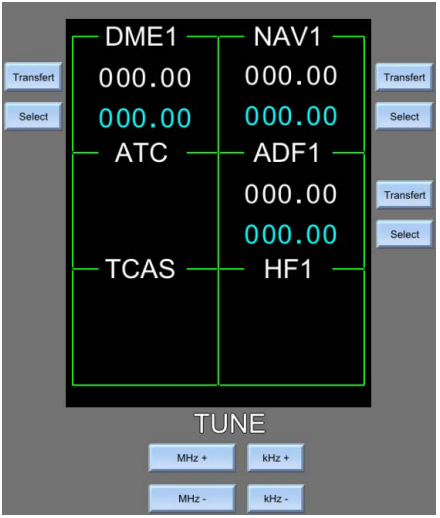
\includegraphics[width=0.6\linewidth]{img/Radio-page.PNG}
            \caption{Radio page}
        \end{figure}
        \begin{figure}[H]
            \centering
            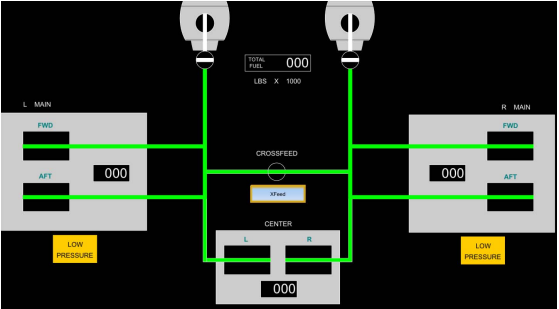
\includegraphics[width=0.6\linewidth]{img/Fuel.PNG}
            \caption{Fuel page}
        \end{figure}